\chapter{Thermal field theory}
\label{chap:tft}

\newcommand{\transampl}{\Braket{\phi_B | e^{- i \hat{H} T / \hbar} | \phi_A}}

In this chapter, we will develop a theory for studying quantum fields at finite temperature $T$.
We will see that there is an elegant mathematical analogy between the path integral for the transition amplitude of a process and the partition function $Z$ of statistical mechanics, allowing us to express the latter in terms of the former.

In a quantum system in the grand canonical ensemble, the partition function is \cite[equation 4.23]{ref:altland_simons}
\begin{equation}
	Z = \trace \left[ e^{-\beta (\hat{H} - \mu_i \hat{N}_i)} \right] = e^{-\beta \Omega} ,
\label{eq:tft:partition_function}
\end{equation}
where $\hat{H}$ is the Hamiltonian operator, $\beta = 1 / k_B T$ is the inverse temperature, $\mu$ is the chemical potential, $\hat{N}_i$ are number operators and $k_B$ is the Boltzmann constant.
The trace can be evaluated in any basis.
If we find $\log Z$, then we have established the link to thermodynamics with the grand potential $\Omega = -k_B T \log{Z}$, and can obtain thermodynamic observables such as 
\cite[chapter 5]{ref:jensoluf}
\begin{subequations}
\begin{align}
	%\text{the entropy}                     \quad \thermalavg{S}   &= -\pdv{\Omega}{T} \\
	            & \text{the average number of particles} & \thermalavg{N_i} & = k_B T \pdv{\log{Z}}{\mu_i},                    & \label{eq:tft:average_number} \\
	            & \text{the average energy}              & \thermalavg{E}   & = \mu_i \thermalavg{N_i} - \pdv{\log{Z}}{\beta}, & \label{eq:tft:average_energy} \\ % \Omega + T S + \mu_i \thermalavg{N_i} \\
	\text{and } & \text{the         pressure}            &             P    & = \frac{k_B T}{V} \log{Z}.                       & \label{eq:tft:average_pressure} % -\pdv{\Omega}{V}
\end{align}
\end{subequations}
In the Tolman-Oppenheimer-Volkoff equation \eqref{eq:tov}, it is precisely the energy density $\epsilon = \thermalavg{E} / \, V$ expressed in terms of the pressure $P$ that we want to insert.
As all relevant information about a system can be derived from the partition function, we say that we have ``solved the system completely'' once we have found $Z$.

First, we will review how the transition amplitude for a process can be expressed as a path integral.
Then we will show how the partition function $Z$ can be expressed as a path integral by Wick rotating the transition amplitude.
By introducing anti-commuting Grassmann numbers, we will see that the partition function for a fermionic field looks quite similar to the bosonic one, although their mathematical foundation is very different.
Finally, we will explicitly calculate the partition function for a bosonic and fermionic gas.

\textit{This chapter is inspired by references \cite{ref:kapusta}, \cite{ref:altland_simons}, \cite{ref:tft_basics} and \cite{ref:tft_random_note_1}.}

\section{Path integral for bosonic partition function}
\label{sec:tft:path_integral_boson}

%TODO: should i have a $t$ as in $\ket{\phi(t)}$ ?)

In this section, we will find a path integral representation of the partition function \eqref{eq:tft:partition_function} for bosons.
First, we will review some elementary properties of the bosonic field $\phi(\vec{x})$ and the conjugate momentum field $\pi(\vec{x})$.
Then we will review how the transition amplitude between two states can be written as a path integral.
Finally, we will show that we can connect the transition amplitude to the partition function and thereby obtain a path integral representation of it.

Consider a quantum field theory for some field $\phi$ with Lagrangian density $\lagr$.
The conjugate momentum field is defined as
\begin{equation}
	\pi = \fdv{\lagr}{\dot\phi} .
\label{eq:tft:conjugate_mometum_definition}
\end{equation}
In the Schrödinger picture, the quantized fields have field operators $\hat{\phi}(\vec{x})$ and $\hat{\pi}(\vec{x})$, and the Hamiltonian operator is
\begin{equation}
	\hat{H} = \int \dif^3 x \, \ham \left( \hat{\pi}(\vec{x}), \hat{\phi}(\vec{x}) \right) ,
\end{equation}
where $\ham = \pi \dot\phi - \lagr$ is the Hamiltonian density obtained from a Legendre transformation of the Lagrangian density.
In analogy with a set of generalized coordinates $q_i$ and momenta $p_i$ in classical mechanics and their corresponding operators $\hat{q}_i$ and $\hat{p}_i$ in quantum mechanics labeled by a discrete index $i$, we can think of $\hat\phi(\vec{x})$ and $\hat\pi(\vec{x})$ as operators in ``position-space'' and ``momentum-space'' labeled by a continuous index $\vec{x}$.
%Whether ``position'' refers to $\vec{x}$ or $\phi(\vec{x})$ will therefore depend on context.

The field operators $\hat{\phi}(\vec{x})$ and $\hat{\pi}(\vec{x})$ have eigenstates $\ket{\phi}$ and $\ket{\pi}$ with corresponding eigenvalues $\phi(\vec{x})$ and $\pi(\vec{x})$ at every point $\vec{x}$, as expressed by the eigenvalue equations
\begin{equation}
	\hat{\phi}(\vec{x}) \ket{\phi} = \phi(\vec{x}) \ket{\phi}
	\qquad \text{and} \qquad
	\hat{\pi}(\vec{x}) \ket{\pi} = \pi(\vec{x}) \ket{\pi} .
\label{eq:tft:field_eigenvalue_equations}
\end{equation}

By assumption, the field and the momentum satisfy the bosonic commutation relations
\begin{equation}
	\comm{\hat{\phi}(\vec{x})}{\hat{\pi}(\vec{y})} = i \hbar \delta(\vec{x} - \vec{y})
	\qquad \text{and} \qquad
	\comm{\hat{\phi}(\vec{x})}{\hat{\phi}(\vec{y})} = 
	\comm{\hat{\pi}(\vec{x})}{\hat{\pi}(\vec{y})} = 
	0 .
\label{eq:tft:boson_field_commutators}
\end{equation}
% peskin eq. 2.20: in Heisenberg picture, these hold at *equal times*

We take the position-space eigenstates to be orthogonal and complete in the sense
\begin{equation}
	\braket{\phi | \phi'} = \prod_{\vec{x}} \delta \left( \phi(\vec{x}) - \phi'(\vec{x}) \right)
	\qquad \text{and} \qquad
	\int \dif \phi \ket{\phi} \bra{\phi} = \1 .
	\label{eq:tft:orthogonality_completeness_position}
\end{equation}

\newcommand{\posmom}[2]{\exp \left[  \frac{i}{\hbar} \int \dif^3 x \, #2(\vec{x}) #1(\vec{x}) \right]}
\newcommand{\mompos}[2]{\exp \left( -\frac{i}{\hbar} \int \dif^3 x \, #1(\vec{x}) #2(\vec{x}) \right)}
If we find the inner product $\braket{\phi | \pi}$, we can use it together with the completeness relation \eqref{eq:tft:orthogonality_completeness_position} to express position-space states and momentum-space states in terms of each other through
\begin{equation}
	\ket\pi = \int \dif \phi \ket\phi \braket{\phi | \pi} %= \int \dif \phi \posmom{\phi}{\pi}
	\qquad \text{and} \qquad
	\ket\phi = \int \dif \pi \ket\pi \braket{\pi | \phi} . %= \int \dif \phi \mompos{\pi}{\phi} .
\end{equation}
To do so, let us use the position-space representation $\hat{\pi} = (\hbar / i) \fdv{}/{\phi}$ of the momentum operator.
This gives us a first-order differential equation
\begin{equation}
	\braket{\phi | \hat{\pi} | \pi} = \pi(\vec{x}) \braket{\phi | \pi} = \frac{\hbar}{i} \fdv*{\braket{\phi | \pi}}{\phi}
\end{equation}
for the inner product $\braket{\phi | \pi}$.
Choosing the solution with prefactor $1$, we obtain
\begin{equation}
	\braket{\phi | \pi} = \posmom{\phi}{\pi} .
	\label{eq:tft:inner_product_position_momentum}
\end{equation}

The momentum states are also orthogonal and complete, but with slightly different factors.
Using the Fourier transformation convention
\begin{equation}
	f(x) = \int \frac{\dif k}{2 \pi} \, e^{-i k x} \hat{f}(k)
	     = \int \dif x' \underbrace{\int \frac{\dif k}{2 \pi} \, e^{i k (x'-x)}}_{\delta(x'-x)} f(x') ,
\end{equation}
we have the Delta function $\delta(x'-x) = \int (\dif k / 2 \pi) \, e^{i k (x'-x)}$, so orthogonality takes the form
\begin{equation}
\begin{split}
	\braket{\pi_a | \pi_b} &= \int \dif \phi \braket{\pi_a | \phi} \braket{\phi | \pi_b} \\
	                       &= \int \dif \phi \exp \left\{ \frac{i}{\hbar} \int \dif^3 x \, \left[ \pi_b(\vec{x}) - \pi_a(\vec{x}) \right] \phi(\vec{x}) \right\} \\
	                       &= 2 \pi \hbar \, \delta \big( \pi_a(\vec{x}) - \pi_b(\vec{x}) \big) .
\end{split}
\end{equation}
To find the completeness relation for $\hat\pi(\vec{x})$, we postulate it up to a constant $B$.
Consider
%Inserting a complete set of both position and momentum states and using the inner product \eqref{eq:tft:inner_product_position_momentum}, consider
\begin{equation}
\begin{split}
	1 &= \int \frac{\dif \pi(\vec{x})}{B} \ket{\pi} \bra{\pi} \\
	  &= \int \frac{\dif \pi(\vec{x})}{B} \ket{\pi} \int \frac{\dif \pi'(\vec{x})}{B} \int \dif \phi(\vec{x}) \braket{\pi | \phi} \braket{\phi | \pi'} \bra{\pi'} \\
	  &= \int \frac{\dif \pi(\vec{x})}{B} \ket{\pi} \int \frac{\dif \pi'(\vec{x})}{B} \underbrace{\int \dif \phi(\vec{x}) \exp \left\{ \frac{i}{\hbar} \int \dif^3 x \, \left[ \pi'(\vec{x}) - \pi(\vec{x}) \right] \phi(\vec{x}) \right\}}_{2 \pi \hbar \, \delta \left( \pi'(\vec{x}) - \pi(\vec{x}) \right)} \bra{\pi'} \\
	  &= \frac{2 \pi \hbar}{B} \underbrace{\int \frac{\dif \pi(\vec{x})}{B} \ket{\pi} \bra{\pi}}_{1} .
\end{split}
\end{equation}
This would be inconsistent unless $B = 2 \pi \hbar$, so completeness in momentum-space is
\begin{equation}
	\int \frac{\dif \pi(\vec{x})}{2 \pi \hbar} \ket{\pi} \bra{\pi} = 1 .
\end{equation}

Let us use these properties to demonstrate how a transition amplitude between two states can be written as a path integral.
When the Hamiltonian $\hat{H}$ is independent of time, a quantum system evolves from an initial state $\ket{\phi_A}$ to the state $\smash[b]{e^{-i \hat{H} T / \hbar}} \ket{\phi_A}$ during the time $T$. \cite[equation 2.28]{ref:sakurai}
Later we will study statistical mechanics for a star in thermal equilibrium -- then the Hamiltonian is always independent of time, otherwise the system would not be in equilibrium.
The transition amplitude for going from the state $\ket{\phi_A}$ to a different state $\ket{\phi_B}$ in the time $T$ is therefore
\begin{equation}
	\transampl \qquad (A \rightarrow B) .
	\label{eq:tft:transition_amplitude_intro}
\end{equation}
Now split the time interval $T$ into $N$ intervals $\Delta t = T / N$, and decompose the evolution operator $e^{- i \hat{H} T / \hbar}$ into equally many products of $e^{- i \hat{H} \Delta t / \hbar}$ to write
\newcommand\pointarrow[1]{\underset{\underset{\displaystyle #1}{\displaystyle \uparrow}}{}}
\begin{equation}
	\transampl = \Braket{\phi_B | e^{- i \hat{H} \Delta t / \hbar} \cdots e^{- i \hat{H} \Delta t / \hbar} \cdots e^{- i \hat{H} \Delta t / \hbar} | \phi_A} .
\label{eq:tft:time_evolution_splitting}
\end{equation}
%\transampl = \braket{\phi_b | \pointarrow{4} e^{- i H \Delta t} \,\, \cdots \pointarrow{3} e^{- i H \Delta t} \pointarrow{2} \cdots \,\, e^{- i H \Delta t} \pointarrow{1} | \phi_a}
We will take the limit $N \rightarrow \infty$ in the end, so we assume that each interval $\Delta t$ is small.
Now comes the most important trick -- take a deep breath and do the following:
\begin{itemize}
\item Insert $N$ complete sets of \emph{momentum} states $1 = \int \dif \pi_n / (2 \pi \hbar) \ket{\pi_n} \bra{\pi_n}$ to the \emph{left} of every exponential, including the rightmost one, with $n$ increasing from right to left.
\item Insert $N-1$ complete sets of \emph{position} states $1 = \int \dif \phi_n \ket{\phi_n} \bra{\phi_n}$ to the \emph{right} of every exponential, excluding the rightmost one, with $n$ increasing from right to left.
\end{itemize}
Now exhale.
With this trick, the transition amplitude can be written as the product
\begin{equation}
	\transampl = \prod_{n=0}^{N} \int \dif \phi_n \int \frac{\dif \pi_n}{2 \pi \hbar} 
	             \Braket{\phi_{n+1} | \vphantom{e^{\hat{H}}} \pi_n} \Braket{\pi_n | e^{- i \hat{H} \Delta t / \hbar} | \phi_n} ,
\label{eq:tft:transition_amplitude_product}
\end{equation}
where we have defined the first and last states
\begin{equation}
	\ket{\phi_0} = \ket{\phi_A}
	\qquad \text{and} \qquad
	\ket{\phi_{N+1}} = \ket{\phi_B}.
\label{eq:tft:bosonic_end_states}
\end{equation}
The inner products $\braket{\phi_{n+1} | \pi_n}$ can simply be replaced by the exponential \eqref{eq:tft:inner_product_position_momentum}, so let us turn our attention to the matrix elements $\braket{\pi_n | e^{- i \hat{H} \Delta t / \hbar} | \phi_n}$.
Since the time step $\Delta t$ is assumed to be small, we can expand the exponential $e^{- i \hat{H} \Delta t / \hbar} \taylor 1 - i \hat{H} \Delta t / \hbar$ to first order in time.
Under the assumption that the Hamiltonian $\hat{H}$ is a sum of terms with all \emph{position}-space operators $\hat{\phi}$ on the \emph{right} and all \emph{momentum}-space operators $\hat{\pi}$ on the \emph{left}, we can pull it out of the product at the additional benefit of replacing its operators by their eigenvalues.
We then obtain
\begin{equation}
\begin{split}
	\Braket{\pi_n | e^{- i \hat{H} \Delta t / \hbar} | \phi_n} &\taylor \Braket{\pi_n | (1 - i \hat{H} \Delta t / \hbar) | \phi_n} \\
	                                                           &=       \Braket{\pi_n | \phi_n} (1 - i H_n \Delta t / \hbar) \\
	                                                           &\taylor \Braket{\pi_n | \phi_n} e^{- i H_n \Delta t / \hbar}, \\
\end{split}
\label{eq:tft:path_integral_hamiltonian_assumption}
\end{equation}
where we no longer have any operators, but only the Hamiltonian eigenvalue at the $n$-th timestep,
\begin{equation}
	H_n = \int \dif^3 x \, \ham \left( \pi_n(\vec{x}), \phi_n(\vec{x}) \right) .
\label{eq:tft:hamiltonian_eigenvalues}
\end{equation}
Since the Hamiltonian $\hat{H} = \hat{H}^\dagger$ is Hermitian, this is still valid if the operators are ordered right-to-left instead of left-to-right.
The left-right from $\hat{\pi}$ to $\hat{\phi}$ order was only assumed for pedagogical reasons to match the left $\bra{\pi_n}$ and right $\ket{\phi_n}$ in \cref{eq:tft:path_integral_hamiltonian_assumption}.
We will only study Hamiltonians that is fully left-right or right-left ordered, for which these steps are valid.
Note the importance of expanding the exponential to first order in time only.
If the Hamiltonian contained \emph{any} mixed sequence of operators such as $H \propto \hat{\pi} \hat{\phi}$, then higher powers like $\hat{H}^2 \propto \hat{\pi} \hat{\phi} \hat{\pi} \hat{\phi}$ in the power series expansion of the time evolution operator would not be in the assumed left-right order.

\iffalse
(TODO: If the Hamiltonian is \emph{not} in the order we assumed above, we could always bring it into this order by commuting operators using the commutation relation \eqref{eq:tft:boson_field_commutators}.
But such terms would appear only as a constant phase on the right side of \eqref{eq:tft:path_integral_hamiltonian_assumption} that would not depend on the dynamics of the process.
AHence, we can relax this assumption by absorbing this physically irrelevant phase into the transition amplitude. ER DETTE RIKTIG? INGEN LÆREBØKER NEVNER DETTE.)

(TODO: if this argument holds, then it can be applied for any $\hat{H}^n$, and there is no reason to expand to first order in time, either)
\fi

\begin{figure}
\centering
\tikzsetnextfilename{phase-space}
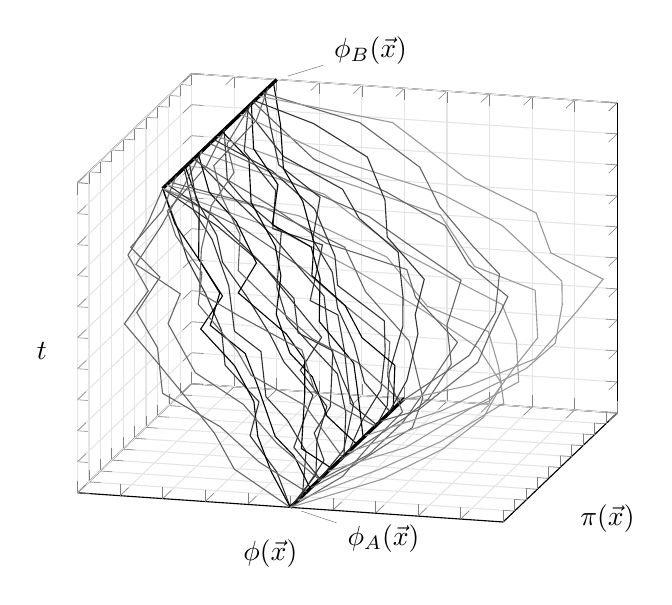
\begin{tikzpicture}
\begin{axis}[
	clip=false,
	view={-75}{20}, 
	%xtick=\empty, ytick=\empty, ztick=\empty, 
	xticklabel=\empty, yticklabel=\empty, zticklabel=\empty,
	xlabel=$\pi(\vec{x})$, ylabel=$\phi(\vec{x})$, zlabel=$t$, zlabel style={rotate=-90},
	%x label style={at={(axis description cs:0.5,0.0)},anchor=north},
	%y label style={at={(axis description cs:0.5,0.0)},anchor=north},
	%z label style={at={(axis description cs:0.5,0.0)},anchor=north},
	xmin=0, xmax=1, ymin=0, ymax=1, zmin=0, zmax=5,
	xtick distance=0.1, ytick distance=0.1, ztick distance=0.5, grid=major, grid style={solid, thin, black!10!white},
	%extra x ticks={0j
	declare function={
		phi1 = 0.5;
		phi2 = 0.8;
		randbetween(\a,\b) = \a + (\b - \a) / 2 * rand;
		%randradius(\x, \rmin, \rmax) = randbetween(\rmin, \rmax) * (\x-0) * (\x-1);
		randfunc(\x,\rmin,\rmax) = randbetween(\rmin,\rmax) * (\x-0)*(\x-1) * 4; % and(x>=0.01, x<=0.99); %(\x-0) * (\x-1);
	},
]
\addplot3 [domain=0:1, samples=2, very thick] ({x}, {phi1}, {0}) node [pos=0.0,pin={-8:$\phi_A(\vec{x})$}] {};
\addplot3 [domain=0:1, samples=2, very thick] ({x}, {phi2}, {5}) node [pos=1.0,pin={+5:$\phi_B(\vec{x})$}] {};
\pgfplotsinvokeforeach{0.0, 0.2, ..., 1.0} {
	\addplot3 [domain=0:1, samples=10, domain y=0:1, samples y=1, black!60!white]  ({max(0, min(1, #1+randbetween(-0.1,0.1))}, {phi1 + (phi2-phi1)*x + randfunc(x,-0.2,-0.3)}, {5*x});
	\addplot3 [domain=0:1, samples=10, domain y=0:1, samples y=1, black!80!white]  ({max(0, min(1, #1+randbetween(-0.1,0.1))}, {phi1 + (phi2-phi1)*x + randfunc(x,-0.0,-0.1)}, {5*x});
	\addplot3 [domain=0:1, samples=10, domain y=0:1, samples y=1, black!100!white] ({max(0, min(1, #1+randbetween(-0.1,0.1))}, {phi1 + (phi2-phi1)*x + randfunc(x,+0.0,+0.1)}, {5*x});
	\addplot3 [domain=0:1, samples=10, domain y=0:1, samples y=1, black!80!white]  ({max(0, min(1, #1+randbetween(-0.1,0.1))}, {phi1 + (phi2-phi1)*x + randfunc(x,+0.2,+0.3)}, {5*x});
	\addplot3 [domain=0:1, samples=10, domain y=0:1, samples y=1, black!60!white]  ({max(0, min(1, #1+randbetween(-0.1,0.1))}, {phi1 + (phi2-phi1)*x + randfunc(x,+0.4,+0.5)}, {5*x});
	\addplot3 [domain=0:1, samples=10, domain y=0:1, samples y=1, black!40!white]  ({max(0, min(1, #1+randbetween(-0.1,0.1))}, {phi1 + (phi2-phi1)*x + randfunc(x,+0.6,+0.7)}, {5*x});
	%\addplot3 [domain=0:1, samples=10, domain y=0:1, samples y=1] ({#1+randfunc(x,0.2,0.3)}, {phi1 + (phi2-phi1)*x + randfunc(x,0.1,0.2)}, {5*x});
}
\end{axis}
\end{tikzpicture}
\caption{\label{fig:phase_space}A quantum system that evolves from the initial field $\phi_A(\vec{x})$ to the final field $\phi_B(\vec{x})$ can take all possible paths through phase space, but some are more likely than others. The conjugate momentum field $\pi(\vec{x})$ does not need to be the same at the start and the end.}
\end{figure}

Substituting \cref{eq:tft:inner_product_position_momentum,eq:tft:path_integral_hamiltonian_assumption,eq:tft:hamiltonian_eigenvalues}, the transition amplitude \eqref{eq:tft:transition_amplitude_product} becomes
\begin{equation}
\begin{split}
	\transampl &=      \left( \prod_{n=1}^N \int \dif \phi_n \int \frac{\dif \pi_n}{2 \pi \hbar} \right) \\
	           &\times \exp \left\{ \frac{i \Delta t}{\hbar} \sum_{n=1}^N \int \dif^3 x \left[ \pi_n(\vec{x}) \frac{\phi_{n+1}(\vec{x}) - \phi_n(\vec{x})}{\Delta t} - \ham \left( \pi_n(\vec{x}), \phi_n(\vec{x}) \right) \right]
	\right\}
	.
\end{split}
\end{equation}
Finally, we take the continuum limit by sending $N \rightarrow \infty$.
It is then natural to define
$\phi(\vec{x}, t_n) = \phi_n(\vec{x}, t_n)$
and
$\pi(\vec{x}, t_n) = \pi_n(\vec{x}, t_n)$
to be the spatial fields at each timestep $t_n$.
Both become continuous functions of time in the continuum limit.
We also use the finite difference definition of the derivative to turn the fraction in the exponential into a partial derivative $\dot{\phi}(\vec{x},t) = \pdv{\phi(\vec{x},t)}/{t}$.
Similarly, we use the Riemann sum definition of the integral to turn the sum $\Delta t\sum$ into an integral $\int \dif t$.
We also define the \textbf{functional integrals}
\begin{equation}
	\int \pathintdif \phi = \lim_{N \rightarrow \infty} \prod_{n=1}^{N} \int \dif \phi_n
	\qquad \text{and} \qquad
	\int \pathintdif \pi = \lim_{N \rightarrow \infty} \prod_{n=1}^{N} \int \frac{\dif \pi_n}{2 \pi \hbar} .
\label{eq:tft:functional_integral}
\end{equation}
%We have swept the diverging factor $(2 \pi \hbar)^N$ under the rug, arguing that it contains no physical information about the dynamics of the process and can be ignored, unlike the other factors.
%TODO: can integrate out momentum with gaussian integral if it appears as $p^2$)
With all of these steps, the transition amplitude takes the form of the \textbf{path integral}
\begin{equation}
\begin{split}
	\transampl &=      \int \pathintdif \pi \int_{\phi(\vec{x}, 0)=\phi_A(\vec{x})}^{\phi(\vec{x},T)=\phi_B(\vec{x})} \pathintdif \phi \\
	           &\times \exp \left\{ \frac{i}{\hbar} \int_0^T \dif t \int \dif^3 x \left[ \pi(\vec{x}, t) \dot{\phi}(\vec{x}, t) - \ham \left( \pi(\vec{x}, t), \phi(\vec{x}, t) \right) \right] \right\} .
\end{split}
\label{eq:tft:path_integral_hamiltonian}
\end{equation}

It is tempting to recognize $\pi \dot\phi - \ham$ as the Legendre transformation that converts to the Lagrangian density and write $\lagr$ in its place.
But we should be careful -- the Legendre transformation converts the independent variable $\dot\phi$ in $\lagr(\phi, \dot\phi, \nabla\phi)$ to $\pi$ in $\ham(\phi, \pi, \nabla\phi)$.
We are integrating over $\pi$ and should therefore not lose track of it by writing $\lagr = \lagr(\phi, \dot\phi, \nabla\phi)$.
Thus, we do not modify the integral further.

\iffalse
Note that the combination of the Hamiltonian and the fields in the exponential is precisely the Legendre transformation that converts between the Hamiltonian density $\ham$ and the Lagrangian density $\lagr$.
Thus, we might as well express the transition amplitude as the \textbf{path integral}
%	\transampl = \int \pathintdif \pi \int_{\phi_A(\vec{x}, 0)}^{\phi_B(\vec{x}, T)} \pathintdif \phi \\
%	             \exp \left( i \int_0^T \dif t \int \dif^3 x \, \left( \lagr(\pi(\vec{x}, t), \phi(\vec{x}, t)) \right) \right) .
\begin{equation}
	\transampl = \int \pathintdif \pi \int_{\phi_A(\vec{x})}^{\phi_B(\vec{x})} \pathintdif \phi \, \exp \big( i S \left[ \pi(\vec{x}, t), \phi(\vec{x}, t) \right] / \hbar \big) ,
\label{eq:tft:path_integral_lagrangian}
\end{equation}
with the action
\begin{equation}
	S \left[ \pi(\vec{x}, t), \phi(\vec{x}, t) \right] = \int_0^T \dif t \int \dif^3 x \, \lagr \left( \pi(\vec{x}, t), \phi(\vec{x}, t) \right) . \qquad \text{TODO: factor $c$?}
\label{eq:tft:action}
\end{equation}
\fi
The path integral expresses the transition amplitude for the process $A \rightarrow B$ as a sum over all possible paths through phase space, each weighted by the value on the unit circle with phase corresponding to the action of the path.
This interpretation is illustrated in \cref{fig:phase_space}.
Note that the position-space integral $\int \pathintdif \phi$ is constrained to start and end in the initial and final states due to the leftmost and rightmost products with the states \eqref{eq:tft:bosonic_end_states}, but the momentum integral $\int \pathintdif \pi$ has no such constraint.

Why have we spent so much time on this transition amplitude, when we really are only interested in the partition function \eqref{eq:tft:partition_function}?
If we evaluate the trace \eqref{eq:tft:partition_function} in the basis of fields $\ket{\phi_0}$, we obtain
\begin{equation}
	Z = \int \dif \phi_0 \Braket{\phi_0 | e^{-\beta (\hat{H} - \mu_i \hat{N}_i)} | \phi_0} .
\end{equation}
This is precisely an integral over transition amplitudes \eqref{eq:tft:path_integral_hamiltonian}, but now with 
\begin{itemize}
\item equal start and end states $\ket{\phi_A} = \ket{\phi_B} = \ket{\phi_0}$, 
\item the Hamiltonian $\hat{H} - \mu_i \hat{N}_i$ and 
\item a purely imaginary time variable $t = -i \tau$ with $\tau$ running from $0$ to $\beta \hbar$.
\end{itemize}
Thus, we can express the partition function \eqref{eq:tft:path_integral_hamiltonian} as path integrals \eqref{eq:tft:path_integral_hamiltonian} with these simple substitutions!
We redefine the field $\phi(\vec{x}, t) \rightarrow \phi(\vec{x}, \tau)$ to be functions of the new ``inverse temperature time'' $\tau$.
Therefore, we substitute $i \int \dif t \rightarrow \int \dif \tau$ and $\dot\phi(x, t) = \pdv{\phi(\vec{x},t)}/{t} \rightarrow \pdv{\phi(\vec{x},\tau)}/{(-i \tau)} = i \dot\phi(\vec{x},\tau)$.
Omitting the arguments of the fields from now, we obtain
\begin{equation}
	Z = \int \pathintdif \pi \oint_+ \pathintdif \phi \, \exp \left[ \frac{1}{\hbar} \int_0^{\beta \hbar} \dif \tau \int \dif^3 x \left( i \pi \dot{\phi} - \ham + \mu \numdensity \right) \right]
\label{eq:tft:bosonic_partition_function}
\end{equation}
where we have absorbed $\int \dif \phi_0$ into the path integral $\int \pathintdif \phi$ and write $\oint_+$ to indicate that we integrate over all fields $\phi(x, \tau) = \phi(x, \tau + \beta \hbar)$ that are \emph{periodic} in $\tau$, due to the equal start and end states $\phi_A(\vec{x}) = \phi_B(\vec{x})$ in \cref{eq:tft:path_integral_hamiltonian}.
Thus, thermal field theory -- statistical mechanics for quantum fields at finite temperature -- is essentially equivalent to ordinary quantum field theory with temperature-dependent time and periodic fields, and the partition function is obtained by integrating along closed paths in phase space!

% inspiration:
% https://physics.stackexchange.com/questions/363666/chemical-potential-in-quantum-field-theories (chemical potential in QFT)
% https://physics.stackexchange.com/questions/294783/rotating-away-a-constant-gauge-field (cannot have single-valued gauge transformation)
% https://physics.stackexchange.com/questions/231092/general-principles-require-that-a-massless-vector-couple-to-a-conserved-current (gauge transformation leaves lagrangian invariant)
The only ingredients in the path integral we have not yet discussed are the chemical potential $\mu$ and the number density $\numdensity$.
In statistical mechanics, we can associate a chemical potential $\mu$ with any conserved quantity $N$ of the system in the ``shifted Hamiltonian'' $H' = H - \mu N$.
How can we connect this to the field theory under study?
Suppose that the field theory admits a conserved current
\begin{equation}
	j^\nu(x)
	\text{ with }
	\partial_\nu j^\nu(x) = 0
	\text{ and conserved charge }
	Q = \int \dif^3 x \, j^0(x)
	\text{ with }
	\odv{Q}{t} = 0.
\end{equation}
In the corresponding quantized quantum field theory, this is equivalent to the commutation $\comm{\hat{H}}{\hat{Q}} = 0$ between the Hamiltonian operator and charge operator.
Then $\odv{\thermalavg{Q}}/{t} = \big< \comm{\hat{H}}{\hat{Q}} \big> = 0$ by the Ehrenfest theorem.
The conserved current $j^\nu(x)$ can be coupled to a gauge field $A_\nu(x)$ by adding the term $A_\nu(x) j^\nu(x)$ to the Lagrangian density $\lagr$, or $-A_\nu(x) j^\nu(x)$ to the Hamiltonian density $\ham$.
Under a standard, Abelian gauge transformation
\begin{equation}
	A_\nu(x) \quad \rightarrow \quad A'_\nu(x) = A_\nu(x) + \partial_\nu \lambda(x) ,
\label{eq:tft:gauge_transformation}
\end{equation}
we can apply the product rule backwards to show that the Lagrangian density changes as
\begin{equation}
	\lagr = \lagr_0 + A_\nu j^\nu \quad \rightarrow \quad \lagr' = \lagr_0 + A'_\nu j^\nu
	      = \lagr   + (\partial_\nu \lambda) j^\nu
	      = \lagr   + \partial_\nu (\lambda j^\nu) - \lambda \partial_\nu j^\nu .
\end{equation}
Thus, the Lagrangian is invariant up to the surface term $\partial_\nu (\lambda j^\nu)$, provided that the current is conserved according to $\partial_\nu j^\nu = 0$, so the equations of motion are unchanged.
To make contact between the field theory and the grand canonical ensemble where $\ham' = \ham - \mu \numdensity$, we see that the chemical potential $\mu$ is equivalent to the temporal component of a constant gauge field
\begin{equation}
	A_\nu(x) = \mu \delta\indices{^0_\nu} 
	\quad \text{coupled to the conserved current} \quad
	\numdensity(x) = j^0(x)!
\label{eq:tft:chemical_potential}
\end{equation}
In conclusion, the so far unspecified density $\numdensity$ in the partition function is identified with the charge density $j^0$ corresponding to the conserved charge $Q = \int \dif^3 x \, j^0(x)$.

To what extent is this coupling physical?
In other words, is it possible to remove the gauge field $A_\nu$ with a gauge transformation \eqref{eq:tft:gauge_transformation} such that $A'_\nu = 0$?
To achieve this, we would have to choose $\lambda(x) = -ct \mu$ up to a constant, because then $A'_\nu = \delta\indices{^0_\nu} \mu + \delta\indices{^0_\nu} \partial_0 \lambda = \mu - \mu = 0$.
But the gauge function $\lambda(t, \vec{x}) \neq \lambda(t + \beta \hbar, \vec{x})$ is not single-valued on the \emph{periodic} manifold of fields we are considering.
We therefore conclude that the gauge transformation is ill-defined, and that the coupling between the chemical potential and conserved current is truly physical.

Later, we will see examples of theories both with and without conserved charges.
When studying Dirac fermions, we will see that the conserved charge corresponds to the difference between the number of particles and antiparticles.
The associated chemical potential essentially functions as a knob with which we can regulate the balance between particles and antiparticles in the system.

% for Abelian theories, we are restricted to introduce chemical potentials only for commuting components of conserved currents! relevant for quark star EoS?}


\section{Path integral for fermionic partition function}

%\newcommand\creat[1]{\hat\psi^\dagger(\vec{#1})}
%\newcommand\destr[1]{\hat\psi        (\vec{#1})}
\newcommand\creat{\hat\psi^\dagger}
\newcommand\destr{\hat\psi        }

We will now develop a path integral for a fermionic field described by a four-spinor $\psi = [ \psi_0, \psi_1, \psi_2, \psi_3 ]$,
For example, the Dirac Lagrangian is $\lagr = \bar{\psi} (i \hbar c \, \slashed\partial - m c^2) \psi$ with conjugate momentum $\pi = \fdv{\lagr}/{\dot\psi} = i \hbar \psi^\dagger$, so we are instructed to treat the field and its conjugate \emph{independently} in the path integral.
This is not a peculiarity of fermionic fields only -- for a complex scalar field $\phi$, for example, we would also be instructed to treat $\phi$ and $\conj\phi$ separately. 

Why do we need to derive the path integral for fermions separately -- can we not just use the bosonic path integral \eqref{eq:tft:bosonic_partition_function} with the appropriate conjugate momentum?
By assumption, the fermion field operators obey the fermionic \textbf{anti-commutation relations}
\begin{subequations}%
\begin{align}%
	\acomm{\destr_\alpha(\vec{x})}{\destr_\beta(\vec{y})} = \acomm{\creat_\alpha(\vec{x})}{\creat_\beta(\vec{y})} &= 0 , \label{eq:tft:fermion_anticommutator_same} \\
	\acomm{\destr_\alpha(\vec{x})}{\creat_\beta(\vec{y})} = \acomm{\creat_\alpha(\vec{x})}{\destr_\beta(\vec{y})} &= \delta_{\alpha \beta} \delta(\vec{x}-\vec{y}) \label{eq:tft:fermion_anticommutator_diff} ,
\end{align}%
\label{eq:tft:fermion_anticommutators}%
\end{subequations}%
in contrast to the bosonic commutators \eqref{eq:tft:boson_field_commutators}.
In the derivation of the bosonic path integral \eqref{eq:tft:bosonic_partition_function}, we treated the eigenvalues $\phi$ and $\pi$ of the operators $\hat\phi$ and $\hat\pi$ as ordinary numbers.
However, the anti-commutators \eqref{eq:tft:fermion_anticommutators} of the fermionic field operators in fact requires their eigenvalues to anti-commute!
For example,
\begin{equation}
\begin{split}
	\text{if}   \quad & \destr \ket{\psi} = \psi \ket{\psi} \quad \text{and} \quad \bra{\psi} \creat = \bra{\psi} \conj\psi , \\
	\text{then} \quad & \braket{\psi | \creat \destr | \psi} = \braket{\psi | \conj\psi \psi | \psi} = -\braket{\psi | \psi \conj\psi | \psi} = -\braket{\psi | \destr \creat | \psi} \quad \text{by \eqref{eq:tft:fermion_anticommutators}}, \\
	\text{so}   \quad & \acomm{\psi}{\conj\psi} = 0 . \\
\end{split}
\label{eq:tft:eigenvalues_must_anticommute}
\end{equation}
By replacing only one operator with its eigenvalue in the second line, we can also deduce the requirements $\acomm{\psi}{\creat} = \acomm{\psi}{\destr} = 0$.
The bosonic path integral \eqref{eq:tft:bosonic_partition_function} and its derivation is therefore not valid for fermions.

\subsubsection{Grassmann numbers}

To develop the fermionic path integral, we therefore replace the algebra of ordinary commuting numbers in the bosonic case with anti-commuting \textbf{Grassmann numbers}.
We will need only a few basic properties of Grassmann numbers, so let us quickly review them here.

The algebra of a set of $N$ Grassmann numbers $\psi_i$ and their conjugates $\conj\psi_i$ is defined by the anti-commutators
\begin{equation}
	\acomm{\psi_i}{\psi_j} = 
	\acomm{\psi_i}{\conj\psi_j} = 
	\acomm{\conj\psi_i}{\conj\psi_j} = 
	0 .
\label{eq:gnums:anticommutators}
\end{equation}
In particular, this implies that $\psi_i^2 = 0$, so $\psi_i^n = 0$ for any $n \geq 2$.
Functions of Grassmann numbers are defined by their Taylor expansion, but the property $\psi_i^2 = 0$ will always terminate the Taylor series after a finite number of terms.
Thus, the most general function of $N$ Grassmann numbers and their conjugates can be written
\begin{equation}
\begin{split}
	f(\psi) &= A + \sum_i A_i \psi_i + \sum_i B_i \conj\psi_i + \sum_{i,j} A_{ij} \psi_i \psi_j + \sum_{i,j} B_{ij} \psi_i \conj\psi_j + \sum_{i,j} C_{i,j} \conj\psi_i \conj\psi_j \\
	        &+ \ldots + Z_{1 \cdots N} \psi_1 \conj\psi_1 \cdots \psi_N \conj\psi_N .
\end{split}
\label{eq:gnums:function_taylor_series}
\end{equation}
For example, for the exponential function of one Grassmann number $\psi$, only the first two terms survive the Taylor series
\begin{equation}
	\exp(\psi) = \sum_{n=0}^\infty \frac{\psi^n}{n!} = 1 + \psi .
\label{eq:gnums:exponential_taylor_series}
\end{equation}
Integration over Grassmann numbers is defined by
\begin{subequations}
\begin{align}
	\iffalse \pdv{1}{\psi_i}      &= 0,           & \qquad \fi \int \dif \psi_i \, 1      &= 0,            \label{eq:gnums:integration_const} \\
	\iffalse \pdv{\psi_j}{\psi_i} &= \delta_{ij}, & \qquad \fi \int \dif \psi_i \, \psi_j &= \delta_{ij} . \label{eq:gnums:integration_var}   
\end{align}
\end{subequations}
\iffalse
Note that $\int \dif \psi \, f(\psi) = \int \dif \psi \, [f(0) + f'(0) \psi] = f'(0) = \pdv{f(\psi)}/{\psi}$, so integration and differentiation are effectively identical operations.
\fi
These are the Grassmann number properties that we will need.

\subsubsection{Fermionic coherent states}

In the derivation of the bosonic path integral \eqref{eq:tft:bosonic_partition_function}, we relied heavily on using eigenstates of the system to take the trace in \eqref{eq:tft:partition_function}, insert completeness relations and take inner products between eigenstates.
To find analogous ways of doing this with fermionic fields, we will introduce \textbf{fermionic coherent states}.

\iffalse
To compute the fermionic path integral, we must therefore replace the algebra of commuting complex numbers in the bosonic case with the algebra of anticommuting \textbf{Grassmann numbers}.
This algebra was invented by the German mathematician Hermann Grassmann in the 19th century.
His work did not gain much traction at that time.
In fact, the publisher of one of his book once wrote to him that
\emph{``(...) since your work hardly sold at all, roughly 600 copies were used in 1864 as waste paper and the remaining few odd copies have now been sold out, with the exception of the one copy in our library.''}
Grassmann was so disappointed with the reception of his work that he turned to study linguistics the last years of his life.
Today, however, his work on Grassmann numbers is the whole fundament for the construction of the fermionic path integral, and his other work is also very important \TODO{fix}.
We review Grassmann numbers in \TODO{ref appendix}.

For concreteness, consider fermions described by the Dirac Lagrangian
\begin{equation}
	\lagr = \bar{\psi} (i \hbar c \slashed\partial - m c^2) \psi .
\end{equation}
Here, the conjugate momentum turns out to be
\begin{equation}
	\pi = \fdv{\lagr}{\dot\psi} = i \hbar \psi^\dagger ,
\label{eq:tft:dirac_conjugate_momentum}
\end{equation}
so, perhaps confusingly, we are instructed to treat the field and its conjugate as independent variables in the path integral.
\fi

Let us get to work.
Suppose we have a finite number $N$ of Grassmann numbers $\psi_i$ with conjugates $\conj\psi_i$ and as many \textbf{creation} and \textbf{annihilation} operators $\creat_i$ and $\destr_i$.
Right after \cref{eq:tft:eigenvalues_must_anticommute}, we argued that Grassmann numbers anti-commute not only with each other, but also with the operators.
By assumption, we therefore start with all the anti-commutators
\begin{subequations}%
\begin{align}%
	\acomm{\destr_i}{\destr_j} = \acomm{\creat_i}{\creat_j}                                                             &= 0            && \quad \text{(similar operators)} , \label{eq:tft:fermionic_anticommutator_sameops} \\
	\acomm{\destr_i}{\creat_j} = \acomm{\creat_j}{\destr_i}                                                             &= \delta_{i j} && \quad \text{(different operators)} , \label{eq:tft:fermionic_anticommutator_diffops} \\
	\acomm{\psi_i}{\psi_j} = \acomm{\psi_i}{\conj\psi_j} = \acomm{\conj\psi_i}{\conj\psi_j}                             &= 0            && \quad \text{(numbers)} , \label{eq:tft:fermionic_anticommutator_gnums} \\
	\acomm{\psi_i}{\destr_j} = \acomm{\psi_i}{\creat_j} = \acomm{\conj\psi_i}{\destr_j} = \acomm{\conj\psi_i}{\creat_j} &= 0            && \quad \text{(numbers and operators)} . \label{eq:tft:fermionic_anticommutator_gnum_op}
\end{align}%
\label{eq:tft:fermionic_all_anticommutators}%
\end{subequations}%
In other words, all field operators and all Grassmann numbers anti-commute with themselves and each other.
The anti-commutators \eqref{eq:tft:fermionic_anticommutator_sameops} and \eqref{eq:tft:fermionic_anticommutator_diffops} are the discrete analogues of the continuous anti-commutators \eqref{eq:tft:fermion_anticommutator_same} and \eqref{eq:tft:fermion_anticommutator_diff}.
It will be more comfortable to carry out the formalism of fermionic coherent states in the discrete case and then take the continuum limit $\psi_i \rightarrow \psi(\vec{x})$ in the end.

The Fock space of the fermionic field has a \textbf{ground state} or \textbf{vacuum state}
\begin{equation}
	\ket{0, 0, \ldots, 0} = \ket{0}. \\
\end{equation}
If we apply any annihilation operator to the ground state, we get
\begin{equation}
	\destr_i \ket{0} = 0, \quad \text{because} \quad \destr_i \destr_i \ket{0} = -\destr_i \destr_i \ket{0} = 0 \text{ by equation \eqref{eq:tft:fermionic_anticommutator_sameops}}.
\label{eq:tft:destroy_zero}
\end{equation}
On the other hand, we can apply a creation operator to build a \textbf{one-particle state}
\begin{equation}
	\ket{1_i} = \ket{(n_1=0), \ldots, (n_i=1), \ldots, (n_N=0)} = \creat_i \ket{0} .
\label{eq:tft:one_particle_state}
\end{equation}
If we apply the same creation operator again, we get
\begin{equation}
	\creat_i \ket{1_i} = 0, \quad \text{because} \quad \creat_i \creat_i \ket{0} = -\creat_i \creat_i \ket{0} = 0 \text{ by equation \eqref{eq:tft:fermionic_anticommutator_sameops}}.
\label{eq:tft:create_one}
\end{equation}
Applying the corresponding annihilation operator instead, we return to the vacuum
\begin{equation}
	\destr_i \ket{1_i} = \destr_i \creat_i \ket{0} = (1 - \creat_i \destr_i) \ket{0} = \ket{0} .
\label{eq:tft:destroy_one}
\end{equation}
More generally, we can apply any sequence of $n = \sum_i n_i$ different creation operators to the vacuum state to build an \textbf{$n$-particle state}
\begin{equation}
	\ket{n_1, n_2, \ldots, n_N} = \left( \creat_1 \right)^{n_1} \cdots \left( \creat_N \right)^{n_N} \ket{0} .
\label{eq:tft:fermionic_many_particle_state}
\end{equation}
This results in a non-zero state only if all $n_i \in \{0, 1\}$, because $(\creat_i)^2 \ket{0} = -(\creat_i)^2 \ket{0} = 0$ by the anti-commutator \eqref{eq:tft:fermionic_anticommutator_sameops}.
Note that shuffling the sequence of operators in \cref{eq:tft:fermionic_many_particle_state} can change the sign of the state.
To avoid ambiguity in our definition, we simply adopt any ordering convention, such as defining the $n$-particle state to have operators with indices that increase from left to right, as in the equation.

The interpretation of this analysis is that the \textbf{creation operator} $\creat_i$ adds a particle in the state $i$, while the \textbf{annihilation operator} $\destr_i$ removes a particle from the same state.
The restriction that $n_i \in \{0, 1\}$ implies that there can be at most one particle in every state and is called the \emph{Pauli exclusion principle}.
Note that the Fock space has a total of $2^N$ distinct states
\begin{equation}
	\ket{n_1, n_2, \ldots, n_N} \qquad \text{where } n_i \in \{0, 1\} \text{ for all } i = 1, \ldots, N .
\label{eq:tft:fermion_all_states}
\end{equation}

Next, define the \textbf{coherent state}
\begin{equation}
\begin{split}
	\ket{\psi} &= \exp \left( -\sum_i \psi_i \creat_i \right) \ket{0} \\
	           &= \prod_i \exp \left( -\psi_i \creat_i \right) \ket{0} \\
	           &= \prod_i \left( 1 - \psi_i \creat_i \right) \ket{0} \qquad \qquad \big( \text{by Taylor expansion \eqref{eq:gnums:exponential_taylor_series}} \big) .
\end{split}
\label{eq:tft:coherent_state_definition}
\end{equation}
%In the last line, we made use of the Taylor expansion \eqref{eq:gnums:function_taylor_series} of functions of Grassmann numbers.
Applying an annihilation operator to this state gives
\begin{equation}
\begin{aligned}
	%\destr_j \ket{\psi} = \psi_j \ket{0} = \psi_j \ket{\psi} \quad \text{(last because $\psi_j^2=0$)}
	%\destr_j \ket{\psi} = \destr_j \prod_i \left( 1 - \psi_i \creat_i \right) \ket{0} = + \psi_j \destr_j \creat_j \ket{0} = \psi_j \ket{0} .
	\destr_j \ket{\psi} &= \destr_j \prod_i \left( 1 - \psi_i \creat_i \right) \ket{0} && \qquad \big( \text{by \eqref{eq:tft:coherent_state_definition}} \big) \\
	                    &= \phantom{\destr_j} \prod_{i \neq j} \left( 1 - \psi_i \creat_i \right) \destr_j \left( 1 - \psi_j \creat_j \right) \ket{0} && \qquad \big( \text{by \eqref{eq:tft:fermionic_anticommutator_diffops} and \eqref{eq:tft:fermionic_anticommutator_gnum_op}} \big) \\
	                    &= \phantom{\destr_j} \prod_{i \neq j} \left( 1 - \psi_i \creat_i \right) \psi_j \ket{0} && \qquad \big( \text{by \eqref{eq:tft:fermionic_anticommutator_diffops}, \eqref{eq:tft:fermionic_anticommutator_gnum_op}, \eqref{eq:tft:destroy_zero} and \eqref{eq:tft:destroy_one}} \big) \\
	                    &= \phantom{\destr_j} \prod_{i \neq j} \left( 1 - \psi_i \creat_i \right) \psi_j \left( 1 - \psi_j \creat_j \right) \ket{0}   && \qquad \big( \text{by \eqref{eq:tft:fermionic_anticommutator_gnums}} \big) \\
                    	&= \psi_j \prod_i \left( 1 - \psi_i \creat_i \right) \ket{0} && \qquad \big( \text{by \eqref{eq:tft:fermionic_anticommutator_gnums} and \eqref{eq:tft:fermionic_anticommutator_gnum_op}} \big) \\
	                    &= \psi_j \ket{\psi} && \qquad \big( \text{by \eqref{eq:tft:coherent_state_definition}} \big) .
\end{aligned}
\label{eq:tft:coherent_state_eigenvalue}
\end{equation}
In other words, the coherent state $\ket{\psi}$ is an eigenstate of every annihilation operator $\destr_j$ with eigenvalue $\psi_j$!
This is analogous to the bosonic eigenvalue equation \eqref{eq:tft:field_eigenvalue_equations}.
It is the coherent states that we wish to use when taking the trace, inner product and inserting identity operators in the path integral.

First, let us find the inner product between two coherent states.
It is
\begin{equation}
\begin{aligned}
	\iffalse
	\braket{\psi | \psi'} &= \braket{0 | \prod_i (1 - \destr_i \conj\psi_i) \prod_j (1 - \psi'_j \creat_j) | 0} \\
	                      &= \braket{0 | 0} + \sum_{i,j} \braket{0 | \destr_i \conj\psi_i \psi'_j \creat_j | 0}
	                       = \braket{0 | 0} + \sum_{i,j} \conj\psi_i \psi'_j \braket{0 | \destr_i \creat_j | 0} \\
	                      &= \braket{0 | 0} + \sum_{i  } \conj\psi_i \psi'_i
	                       = 1 + \sum_i \conj\psi_i \psi'_i = \exp \left( \sum_i \conj\psi_i \psi'_i \right) .
	\fi
	\braket{\psi | \psi'} %&= \braket{\psi | \prod_i (1 - \psi'_i \creat_i) | 0} && \qquad \big( \text{by \eqref{eq:tft:coherent_state_definition}} \big) \\
	                      %&= \braket{\psi | \prod_i (1 + \creat_i \psi'_i) | 0} && \qquad \big( \text{by \eqref{eq:tft:fermionic_anticommutator_gnum_op}} \big) \\
	                      %&= \braket{\psi | \prod_i (1 + \conj\psi_i \psi'_i) | 0} && \qquad \big( \text{by \eqref{eq:tft:coherent_state_eigenvalue}} \big) \\
	                      &= \braket{\psi | \prod_i (1 + \conj\psi_i \psi'_i) | 0} && \qquad \big( \text{by \eqref{eq:tft:coherent_state_definition}, \eqref{eq:tft:fermionic_anticommutator_gnum_op} and \eqref{eq:tft:coherent_state_eigenvalue}} \big) \\
	                      %&= \braket{0 | \prod_j (1 - \destr_j \conj\psi_j) \prod_i (1 + \conj\psi_i \psi'_i) | 0} && \qquad \big( \text{by the dual of \eqref{eq:tft:coherent_state_definition}} \big) \\
	                      &= \braket{0    | \prod_i (1 + \conj\psi_i \psi'_i) | 0} && \qquad \big( \text{by orthogonality} \big) \\
	                      %&= \underbrace{\braket{0 | 0}}_{1} \prod_i (1 + \conj\psi_i \psi'_i) && \qquad \big( \text{by \eqref{eq:tft:destroy_zero}} \big) \\
	                      &= \exp \left( \sum_i \conj\psi_i \psi'_i \right) && \qquad \big( \text{by $\braket{0|0}=1$ and \eqref{eq:gnums:exponential_taylor_series}} \big) .
\end{aligned}
\label{eq:tft:grassmann_inner_product_discrete}
\end{equation}

Next, we can work out that the unit operator $\1$ can be represented by the integral
\begin{equation}
\begin{split}
	 \iffalse
	 & \int \dif \conj{\psi} \int \dif \psi \, e^{-\sum_i \conj\psi_i \psi_i} \ket{\psi} \bra{\psi} \\
	=& \int \dif \conj{\psi} \int \dif \psi \, \prod_i \left( 1 + \psi_i \conj{\psi}_i \right) \prod_j \left( 1 - \psi_j \creat_j \right) \ket{0} \bra{0} \prod_k \left( 1 - \destr_k \conj\psi_k \right) \\
	=& \int \dif \conj{\psi} \int \dif \psi \, \prod_i \left( 1 + \psi_i \conj{\psi}_i \right) \prod_j \left( 1 - \psi_j \creat_j \right) \ket{0} \bra{0} \left( 1 - \destr_j \conj\psi_j \right) \\
	=& \sum_{n_1=0}^1 \sum_{n_2=0}^1\cdots \sum_{n_N=0}^1 \ket{n_1, n_2, \ldots, n_N} \bra{n_1, n_2, \ldots, n_N} = \1 \\
	=& \int \dif \conj{\psi} \int \dif \psi \left[ \left( -\sum_i \conj{\psi}_i \psi_i \right) \ket{0} \bra{0} + \left( -\sum_j \psi_j \creat_j \right) \ket{0} \bra{0} \left( -\sum_k \destr_k \conj\psi_k \right) \right] \\
	=& \int \dif \conj{\psi} \int \dif \psi \left[ \sum_i \psi_i \conj\psi_i \ket{0} \bra{0} + \sum_{j,k} \psi_j \conj\psi_k \ket{1_j} \bra{1_k} \right] \\
	=& \ket{0} \bra{0} + \sum_j \ket{1_j} \bra{1_j} = \1 . \\
	\fi
	 & \int \dif \conj{\psi} \int \dif \psi \, \exp \left( -\sum_i \conj\psi_i \psi_i \right) \ket{\psi} \bra{\psi} \\
	=& \int \dif \conj{\psi} \int \dif \psi \, \prod_i \Big( 1 + \psi_i \conj{\psi}_i \Big) \prod_j \left( 1 - \psi_j \creat_j \right) \ket{0} \bra{0} \prod_k \left( 1 - \destr_k \conj\psi_k \right) \\
	=& \sum_{n_1=0}^1 \sum_{n_2=0}^1\cdots \sum_{n_N=0}^1 \ket{n_1, n_2, \ldots, n_N} \bra{n_1, n_2, \ldots, n_N} = \1 . \\
\end{split}
\label{eq:tft:completeness_grassmann_discrete}
\end{equation}
To make the big leap across the second equality sign, stare intensely at the middle line while following the next argument.
To get a non-zero contribution from the integral, the parentheses must be multiplied out in a way such that one gets terms with the particular combination
\begin{equation}
	\int \dif \conj\psi \int \dif \psi \, \psi_1 \conj\psi_1 \cdots \psi_N \conj\psi_N = 1 .
\label{eq:tft:integral_saturated}
\end{equation}
Why?
Any term with duplicate fields $\psi_i^2 = -\psi_i^2 = 0$ will yield zero.
Similarly, if a term has a product that does not contain \emph{all} the factors $\psi_1,\, \conj\psi_1,\, \ldots,\, \psi_N,\, \conj\psi_N$, then after integrating out the \emph{present} factors with integral \eqref{eq:gnums:integration_var}, there will always be left behind a vanishing constant integral in the form \eqref{eq:gnums:integration_const} over the \emph{absent} factors, causing the whole integral to vanish.
Based on this, we can derive three rules for what combinations of factors we can choose when multiplying out the three parentheses.
\begin{enumerate}
\item \textbf{For any $i$ in the first parenthesis:} Given that we follow the two next rules, we are free to choose either the factor $1$ or $\psi_i \conj\psi_i$. \label{eq:tft:logic_tree_one}
\item \textbf{For $j=i$ in the second parenthesis:} 
If we choose $\psi_i \conj\psi_i$ in the first parenthesis, we \emph{must} choose $1$ in the second to avoid a duplicate factor $\psi_i^2 = 0$.
Conversely, if we choose $1$ in the first, we \emph{must} choose $-\psi_j \smash[t]{\creat_j}$ in the second to ``saturate'' the product \eqref{eq:tft:integral_saturated}.
\item \textbf{For $k = j = i$ in the third parenthesis:} 
If we choose $-\psi_j \creat_j$ in the second, we \emph{must} choose $\smash{-\psi_k \creat_k}$ in the third to get $\psi_j \conj\psi_j$ in the field product.
Conversely, if we choose $1$ in the second, then we have already included $\psi_i \conj\psi_i$ from rule \ref{eq:tft:logic_tree_one}, and we \emph{must} choose $1$ in the third to avoid a duplicate factor $(\conj\psi_i)^2 = 0$. \label{eq:tft:logic_tree_three}
\end{enumerate}
Following these rules, the first parenthesis expands to all possible $2^N$ terms.
For every one of these terms, there is precisely one combination of factors in the second and third parentheses that yields a nonzero contribution.
This evaluates to $2^N$ terms with all possible combinations of $N_j = N_k$ creation and annihilation operators and $N_i = N - N_j$ Grassmann numbers.
\emph{These $2^N$ terms are therefore precisely all the $2^N$ states \eqref{eq:tft:fermion_all_states} in the Fock space!}
The sign ambiguity following different orderings of operators in the $n$-particle states \eqref{eq:tft:fermionic_many_particle_state} does not cause any problems with signs in the sum over all the states, either.
To understand why, note that rule \ref{eq:tft:logic_tree_three} forces us to apply the \emph{same} sequence of operators to both $\ket{0}$ and $\bra{0}$ in \cref{eq:tft:completeness_grassmann_discrete}, and any ordering that does not follow definition \eqref{eq:tft:fermionic_many_particle_state} can be made to do so by anti-commuting the \emph{same} operators in \emph{both} sequences, introducing an \emph{even} number of minus signs that cancel.
This explains the transition to the final line.
\iffalse
\begin{itemize}
\item choose $k = j$ in the third parenthesis in order to pair $\psi_j$ with $\conj\psi_j$, and
\item for every factor $\psi_i \conj\psi_i$ one chooses from the first parenthesis, one must choose the factor $1$ from the second and third parentheses in order to avoid $\psi_i^2=0$, and conversely,
\item for every factor $1$ one chooses from the first parenthesis, one must choose the factor $-\psi_j \creat_j$ and $-\destr_k \conj\psi_k$ from the second and third parentheses in order to not miss a factor $\psi_i \conj\psi_i$ in the product \TODO{ref}.
\end{itemize}
Following these rules is equivalent to iterating over all $2^N$ combinations with $N_j$ creation and annihilation operators in the second and third parentheses and $N_i = N - N_j$ Grassmann numbers in the first parenthesis.
\fi
%To be clear, the very last equality follows because the sum goes over all states \eqref{eq:tft:fermion_all_states} in the Fock space.

With the same reasoning, we can work out that the trace of an operator $\hat{A}$ can be written
\begin{equation}
\begin{aligned}
	 & \int \dif \conj{\psi} \int \dif \psi \, \exp \left( -\sum_i \conj{\psi}_i \psi_i \right) \braket{-\psi | \hat{A} | \psi} \\
	=& \int \dif \conj{\psi} \int \dif \psi \, \prod_i \Big( 1 + \psi_i \conj\psi_i \Big) \braket{0 | \prod_j \Big( 1 + \destr_j \conj\psi_j \Big) \hat{A} \prod_k \Big( 1 - \psi_k \creat_k \Big) | 0} \\
	%=& \int \dif \conj{\psi} \int \dif \psi \, \prod_i \Big( 1 + \psi_i \conj\psi_i \Big) \braket{0 | \prod_j \Big( 1 + \destr_j \conj\psi_j \Big) \hat{A} \Big( 1 - \psi_j \creat_j \Big) | 0} && \big( \text{$k=j$} \big) \\
	%=& \int \dif \conj{\psi} \int \dif \psi \, \prod_i \Big(1 + \conj\psi_i \psi_i \Big) \prod_j \conj\psi_j \psi_j \braket{0 | (1 + \destr_j \psi_j) \hat{A} (1 + \conj\psi_j \creat_j) | 0} \\
	=& \sum_{n_1=0}^1 \sum_{n_2=0}^1\cdots \sum_{n_N=0}^1 \braket{n_1, n_2, \ldots, n_N | \hat{A} | n_1, n_2, \ldots, n_N} = \trace{\hat{A}} . \\
	%=& \int \dif \conj{\psi} \int \dif \psi \left[ (-\sum_i \conj\psi_i \psi_i) \braket{0 | \hat{A} | 0} + \braket{0 | (+\sum_j \destr_j \conj\psi_j) \hat{A} (-\sum_k \psi_k \creat_k) | 0} \right] \\
	%=& \int \dif \conj{\psi} \int \dif \psi \left[ \sum_i \psi_i \conj\psi_i \braket{0 | \hat{A} | 0} + \sum_{j,k} \psi_k \conj\psi_j \braket{1_j | \hat{A} | 1_k} \right] \\
	%=& \braket{0 | \hat{A} | 0} + \sum_j \braket{1_j | \hat{A} | 1_j} = \trace{\hat{A}} . \\
\end{aligned}
\label{eq:tft:trace_grassmann_discrete}
\end{equation}
The rules for multiplying out the parentheses are virtually identical to those in \cref{eq:tft:completeness_grassmann_discrete}.
Schematically, the two last parentheses give contributions in the form $\smash[b]{\braket{0 | ( \destr_j \conj\psi_j ) \hat{A} ( -\psi_k \creat_k ) | 0}} = + \smash[b]{\psi_k \conj\psi_j \braket{0 | \destr_j \hat{A} \creat_k | 0}}$ and all its multi-particle generalizations, where we must set $j=k$ to get a non-zero contribution.
In addition, we have \emph{assumed} that $\smash{\hat{A}}$ is a ``bosonic'' operator that \emph{commutes} with the Grassmann numbers, allowing us to move the Grassmann numbers out of the inner product in this way.
For example, the Dirac Hamiltonian \eqref{eq:tft:dirac_hamiltonian} that we will work with later is such an $\hat{A}$, as it contains \emph{two} field operators.
\emph{Pay special attention to the minus sign in $\bra{-\psi} = \bra{0} \prod_j [1 - \creat_j (-\psi_j)] = \bra{0} \prod_j [1 + \creat_j \psi_j]$ in the first line!}
Without it, we would not obtain the trace when multiplying out the parentheses.
\emph{We will soon see that this minus sign is perhaps the most important result of this whole chapter, yet surely the least visible one!}

As we remarked at the start, this analysis was for discrete fields that satisfy the discrete anti-commutators \eqref{eq:tft:fermionic_all_anticommutators}.
We are studying fields $\psi(\vec{x})$ and $\conj\psi(\vec{x})$ with an infinite number of field operators $\creat(\vec{x})$ and $\destr(\vec{x})$ that satisfy the continuum generalization \eqref{eq:tft:fermion_anticommutators}.
Our results carry over with the substitutions $\psi_i \rightarrow \psi(\vec{x})$, as if every Grassmann number corresponds to the field at one position, and $\sum_i \rightarrow \int \dif^3 x$.
The continuum version of the coherent state is
\begin{equation}
	\ket{\psi} = \exp \left[ -\int \dif^3 x\, \psi(\vec{x}) \hat\psi^\dagger(\vec{x}) \right] \ket{0} .
\end{equation}
\begin{subequations}
The inner product \eqref{eq:tft:grassmann_inner_product_discrete} between two coherent states is then
\begin{equation}
	\braket{\psi | \psi'} = \exp \left[ \int \dif^3 x \, \conj\psi(\vec{x}) \psi'(\vec{x}) \right] ,
\label{eq:tft:grassmann_inner_product}
\end{equation}
and the identity operator \eqref{eq:tft:completeness_grassmann_discrete} becomes
\begin{equation}
	\int \dif \conj\psi \int \dif \psi \, \exp \left[ -\int \dif^3 x \, \conj\psi(\vec{x}) \psi(\vec{x}) \right] \ket{\psi} \bra{\psi} = \1 ,
\label{eq:tft:completeness_grassmann}
\end{equation}
while the trace \eqref{eq:tft:trace_grassmann_discrete} is modified to 
\begin{equation}
	\int \dif \conj\psi \int \dif \psi \, \exp \left[ -\int \dif^3 x \, \conj\psi(\vec{x}) \psi(\vec{x}) \right] \Braket{-\psi | \hat{A} | \psi} = \trace{\hat{A}} .
\label{eq:tft:trace_grassmann}
\end{equation}
\end{subequations}
The most important thing to note is the necessity of the \emph{minus sign} in $\bra{-\psi}$ of the trace \eqref{eq:tft:trace_grassmann} -- we will see that this requires fermionic fields to be \emph{anti-periodic} in imaginary time, in contrast to the periodic bosonic fields.

\subsubsection{Partition function}

Using equations \eqref{eq:tft:grassmann_inner_product}, \eqref{eq:tft:completeness_grassmann} and \eqref{eq:tft:trace_grassmann} as our toolbox, let us now construct the path integral for the fermionic partition function.
We now revert from the above notation with single fermion fields $\psi$ and $\conj\psi$ back to the four-component spinors $\psi$ and $\psi^\dagger$.
Accordingly, we write $\prod_{\alpha=0}^3 \dif \psi_\alpha = \dif \psi$ and $\prod_{\alpha=0}^3 \dif \conj\psi_\alpha = \dif \psi^\dagger$ to indicate integration over all four components.
The partition function \eqref{eq:tft:partition_function} follows from the trace \eqref{eq:tft:trace_grassmann} with $\smash[t]{\hat{A}} = \smash[t]{e^{-\beta (\hat{H} - \mu \hat{N})}}$ as
\begin{equation}
	Z = \int \dif \psi_0^\dagger \int \dif \psi_0 \, e^{-\int \dif^3 x \, \psi_{0}^\dagger(\vec{x}) \psi_{0}(\vec{x})} \Braket{-\psi_0 | e^{-\beta(\hat{H} - \mu \hat{N})} | \psi_0} .
\label{eq:tft:fermion_path_integral_after_completeness}
\end{equation}
Breaking up the operator $e^{-\beta (\hat{H} - \mu \hat{N})}$ as in \cref{eq:tft:time_evolution_splitting} with small times $\Delta \tau = \beta \hbar / N$ and inserting one Grassmann completeness relation \eqref{eq:tft:completeness_grassmann} between every factor, the partition function becomes
\begin{equation}
	Z = \prod_n \int \dif \psi_n^\dagger \int \dif \psi_n \, e^{-\int \dif^3 x \, \psi_{n+1}^\dagger(\vec{x}) \psi_{n+1}(\vec{x})} \Braket{\psi_{n+1} | e^{-(\hat{H} - \mu \hat{N}) \Delta \tau / \hbar} | \psi_n} ,
\end{equation}
where we defined the left end state
\begin{equation}
	\bra{\psi_{N+1}} = \bra{-\psi_0} \qquad \big( \text{\textbf{note the minus sign!}} \big) .
\label{eq:tft:fermionic_end_state}
\end{equation}
We are hiding the minus sign to be able to write the expression in compact product notation.
Do not forget it!
Next, expand the Hamiltonian to first order as in \cref{eq:tft:path_integral_hamiltonian_assumption}.
Then we obtain
\begin{equation}
	Z = \prod_n \int \dif \psi_n^\dagger \int \dif \psi_n \, e^{-\int \dif^3 x \, \psi_{n+1}^\dagger(\vec{x}) \psi_{n+1}(\vec{x})} \braket{\psi_{n+1} | \psi_n} e^{-(H_n - \mu N) \Delta \tau / \hbar} .
\end{equation}
Now use the Grassmann inner product \eqref{eq:tft:grassmann_inner_product} on $\braket{\psi_{n+1} | \psi_n}$ to write
\begin{equation}
	Z = \prod_n \int \dif \psi_n^\dagger \int \dif \psi_n \, \exp \left[ \frac{\Delta \tau}{\hbar} \sum_n \int \dif^3 x \left( -\hbar \psi^\dagger_{n+1} \frac{\psi_{n+1} - \psi_n}{\Delta \tau} \psi_{n} - \ham + \mu \numdensity \right) \right] .
\end{equation}
% integrate by parts? %why is this valid for Grassmann numbers? Can one e.g. show that $\pdv{\phi^\dagger \phi}{\tau} = 0$?, change order/use int by parts correctly % TODO: don't need this, should rather be careful about index placement above (especially the exp(.. n+1 ..) from completeness)
Finally, take the continuum limit and introduce the functional integrals $\pathintdif \psi = \prod_{n=1}^\infty \dif \psi_n$ and $\pathintdif \psi^\dagger = \prod_{n=1}^\infty \dif \psi^\dagger$. 
We then obtain the \textbf{fermionic partition function}
\begin{equation}
	Z = \oint_- \pathintdif \psi^\dagger \oint_- \pathintdif \psi \exp \left[ \frac{1}{\hbar} \int_0^{\beta \hbar} \dif \tau \int \dif^3 x \left( -\hbar \psi^\dagger \dot{\psi} - \ham \left( \psi^\dagger, \psi \right) + \mu \numdensity \right) \right] ,
\label{eq:tft:fermion_partition_function}
\end{equation}
where $\oint_-$ means to integrate over \emph{anti-periodic} fields $\psi(\vec{x}, 0) = -\psi(\vec{x}, \beta \hbar)$, naturally extending the symbol $\oint_+$ we introduced for bosonic fields that were \emph{periodic}.
Here, anti-periodicity follows from the negative sign in $\bra{-\psi}$ in the trace \eqref{eq:tft:trace_grassmann} that we hid in the end state \eqref{eq:tft:fermionic_end_state}.
Remarkably, this result looks identical to the bosonic partition function \eqref{eq:tft:bosonic_partition_function} with canonical momentum $\pi = i \hbar \psi^\dagger$, despite the very different machinery with anti-periodic Grassmann fields.

\iffalse
The partition function is therefore
\begin{equation}
\begin{split}
	Z &= \int \dif \psi_0^\dagger \int \dif \psi_0 \, e^{-\psi_{n+1}^\dagger \psi_{n+1}} \braket{-\psi_0 | e^{-\beta(\hat{H} - \mu \hat{N})} | \psi_0} \\
	  &= \prod_n \int \dif \psi_n^\dagger \int \dif \psi_n \, e^{-\psi_{n+1}^\dagger \psi_{n+1}} \braket{\psi_{n+1} | e^{-(\hat{H} - \mu \hat{N}) \Delta \tau / \hbar} | \psi_n} \\
	  &= \prod_n \int \dif \psi_n^\dagger \int \dif \psi_n \, e^{-\psi_{n+1}^\dagger \psi_{n+1}} \braket{\psi_{n+1} | \psi_n} e^{-(H_n - \mu N) \Delta \tau / \hbar} \\
	  &= \prod_n \int \dif \psi_n^\dagger \int \dif \psi_n \, \exp \left\{ -\frac{\Delta t}{\hbar} \sum_n \int \dif^3 x \left( \psi^\dagger_{n+1} \frac{\psi_{n+1} - \psi_n}{\Delta t} + \ham - \mu \numdensity \right) \right\} \\
	  &= \oint_- \pathintdif \psi^\dagger \oint_- \pathintdif \psi \exp \left\{ \frac{1}{\hbar} \int_0^{\beta \hbar} \dif \tau \int \dif^3 x \left( -\psi^\dagger(\vec{x},\tau) \dot{\psi}(\vec{x},\tau) - \ham \left( \psi^\dagger(\vec{x},\tau), \psi(\vec{x},\tau) \right) + \mu \numdensity \right) \right\} \\
\end{split}
\end{equation}
\fi

\section{Matsubara frequencies and box quantization}
\label{sec:matsubara_quantization}

We have just seen that the partition function for bosons and fermions can be expressed by path integrals over fields that are periodic and anti-periodic on the time interval $\beta \hbar$, respectively.
In other words, a bosonic \emph{or} fermionic field $\phi(\vec{x}, \tau)$ satisfies the (anti-)periodicity
\begin{equation}
	\phi(\vec{x}, \tau) = \begin{cases}
		+ \phi(\vec{x}, \tau + \beta \hbar) & \text{for bosons} \\
		- \phi(\vec{x}, \tau + \beta \hbar) & \text{for fermions} .
	\end{cases}
\label{eq:tft:periodicity}
\end{equation}
Accordingly, we can expand either field in a Fourier series
\begin{equation}
	\phi(\vec{x}, \tau) = \sum_n \phi_n(\vec{x}) e^{i \omega_n \tau}
\end{equation}
with \textbf{Matsubara frequencies} 
\begin{equation}
	\omega_n = \begin{cases}
		2 \pi n / \beta \hbar    & \text{for bosons} \\
		2 \pi (n+\frac12) / \beta \hbar & \text{for fermions} .
	\end{cases}
\label{eq:tft:matsubara_frequencies}
\end{equation}

The field is not periodic in space, but let us for a moment pretend that it is by putting it in a fictitious box of volume $V = L^3$ and impose periodic boundary conditions.
Then the spatial part of the field can also be represented by a Fourier series
\begin{equation}
	\phi_n(\vec{x}) = \sum_\vec{k} \phi_n(\vec{k}) e^{i \vec{k} \cdot \vec{x}} ,
\end{equation}
where the sum runs over all wavevectors $\vec{k}$ with components $k_i = 2 \pi n_i / L$ for integers $n_i$, each separated by the distance $\Delta k = 2 \pi / L$ in $\vec{k}$-space.
Since the field is not really periodic, we should take the continuum limit $V \rightarrow \infty$ at the end.
Then $\Delta k \rightarrow 0$, so the sum is replaced by the integral
\begin{equation}
	\sum_\vec{k} = 
	\sum_\vec{k} \frac{(\Delta k)^3}{(2 \pi / L)^3} 
	\quad \rightarrow  \quad
	\int \frac{\dif^3 k}{(2 \pi / L)^3} =
	V \int \frac{\dif^3 k}{(2 \pi)^3} .
\label{eq:tft:continuum_limit}
\end{equation}
This mathematical trick is known as \textbf{box quantization}.
In the following sections, we will therefore proceed through a calculation with a finite Fourier series expansion
\begin{equation}
	\phi(\vec{x}, \tau) = \sum_n \sum_\vec{k} \phi_n(\vec{k}) e^{i (\vec{k} \cdot \vec{\vec{x}} + \omega_n \tau)}
\label{eq:tft:fourier_series}
\end{equation}
of the field, then take the continuum limit \eqref{eq:tft:continuum_limit} at the end of the calculation to make it physically correct.

The infinite volume factor $V$ will come in handy when calculating thermodynamic observables.
To obtain the pressure \eqref{eq:tft:average_pressure}, we are instructed to divide by volume.
Similarly, we will need to divide by volume to convert extensive observables like the energy \eqref{eq:tft:average_energy} into intensive observables like the energy \emph{density} $\epsilon = \thermalavg{E} / \, V$ that we need in the Tolman-Oppenheimer-Volkoff equation \eqref{eq:tov}.

The wave number $\vec{k}$ and the Matsubara frequency $\omega_n$ here arose due to geometrical considerations of the periodicity of the field.
We will soon see that they have important physical consequences, too.
In anticipation of this, we define the corresponding momentum and Matsubara energy
\begin{equation}
	\vec{p} = \hbar \vec{k}, \qquad
	E_n = \hbar \omega_n \qquad \text{and} \qquad
	\sum_\vec{p} = \sum_\vec{k} = V \int \frac{\dif^3 p}{(2 \pi \hbar)^3}.
\label{eq:tft:matsubara_energies}
\end{equation}

Note that some authors adopt the four-momentum $p = (E_n/c, \vec{p})$ and write the Fourier amplitude as $\phi(p)$.
Due to the difference between the discrete nature of the Matsubara energies and the continuous nature of the momenta, we wish to maintain some ``separation'' between time and space and therefore choose to write $\phi_n(\vec{p})$.

\section{Partition function for free bosonic real scalar field}

As a first example, we apply the path integral formalism to find the partition function for a free real scalar field representing spin-zero bosons.
Its Lagrangian density is
% note: unit of phi is sqrt(energy / length)
\begin{equation}
	\lagr = \frac{1}{2} (\partial_\mu \phi) (\partial^\mu \phi) - \frac12 \frac{m^2 c^2}{\hbar^2} \, \phi^2
	      = \frac{1}{2 c^2} \dot{\phi}^2 - \frac12 (\nabla \phi)^2  - \frac12 \frac{m^2 c^2}{\hbar^2} \, \phi^2 .
\label{eq:tft:boson_lagrangian}
\end{equation}
To be clear, we now denote time by $\tau$, regard the field as a function $\phi(\vec{x}, \tau)$ and denote the time derivative by $\dot{\phantom{\phi}} = \pdv{}/{\tau}$.
There is no $t$ anymore, only the $\tau$ of the path integral \eqref{eq:tft:bosonic_partition_function}.
The conjugate momentum \eqref{eq:tft:conjugate_mometum_definition} is
\begin{equation}
	\pi = \pdv{\lagr}{\dot{\phi}} = \frac{1}{c^2} \dot{\phi} .
\end{equation}
The Hamiltonian density is therefore
\begin{equation}
	\ham = \pi \dot{\phi} - \lagr = \frac12 c^2 \pi^2 + \frac12 (\nabla \phi)^2 + \frac12 \frac{m^2 c^2}{\hbar^2} \phi^2 .
\label{eq:tft:boson_hamiltonian}
\end{equation}
We now calculate the partition function \eqref{eq:tft:bosonic_partition_function}.
To do so, we need the combination
\begin{equation}
\begin{split}
	i \pi \dot\phi - \ham &= i \pi \dot\phi - \frac{1}{2} c^2 \pi^2 - \frac12 (\nabla \phi)^2 - \frac{1}{2} \frac{m^2 c^2}{\hbar^2} \phi^2 \\
	                      &= -\frac{1}{2} c^2 \left( \pi - \frac{i}{c^2} \dot\phi \right)^2 - \frac{1}{2 c^2} \dot\phi^2 - \frac{1}{2} (\nabla \phi)^2 - \frac{1}{2} \frac{m^2 c^2}{\hbar^2} \phi^2 \\
	                      &= -\frac{1}{2} c^2 \tilde\pi^2 + \lagr_E . \\
\end{split}
\label{eq:tft:boson_field_combination}
\end{equation}
We completed the square by defining the shifted field $\tilde\pi = \pi - i \dot\phi / c^2$, for reasons that soon will be apparent.
Remember that the Legendre transformation \eqref{eq:tft:boson_hamiltonian} exchanges the independent variable $\dot\phi$ in $\lagr = \lagr(\phi, \dot\phi, \nabla\phi)$ to $\pi$ in $\ham = \ham(\phi, \pi, \nabla\phi)$.
Thus, the shift can be regarded as a shift by a \emph{constant}.
We also defined the remaining terms as the Lagrangian density $\lagr_E$.
It is exactly the original Lagrangian density \eqref{eq:tft:boson_lagrangian}, only with $\tau \rightarrow i \tau$.
This can be interpreted as a change from Minkowski space to Euclidean space, and we therefore call $\lagr_E(\tau) = \lagr(i \tau)$ the Euclidean Lagrangian density.
The path integral \eqref{eq:tft:bosonic_partition_function} is now
\begin{equation}
	Z = \int \pathintdif \pi \oint_+ \pathintdif \phi \exp \left\{ \frac{1}{\hbar} \int_0^{\beta \hbar} \dif \tau \int_V \dif^3 x \left[ - \frac12 c^2 \tilde\pi^2 + \lagr_E \right] \right\} .
\label{eq:tft:boson_integrate_out_momentum}
\end{equation}
\label{tft:pressure_renormalization_discussion}%
Since $\tilde\pi$ can be regarded as a constant shift of the field $\pi$, we can now use the Gaussian integral \eqref{eq:integrals:gaussian_axx} to \emph{integrate out} the momentum. 
We do not bother keeping track of the resulting constant or any other constants in front of the partition function.
Physical quantities like the energy \eqref{eq:tft:average_energy} only involve derivatives of $\log Z$ and would be unaffected by such constants.
The pressure \eqref{eq:tft:average_pressure}, however, contains $\log Z$ without derivatives and would really be shifted by an infinite constant, due to the infinite number of integrals in the functional integral \eqref{eq:tft:functional_integral}.
It is most correct, therefore, to disregard constants in $Z$ with the attitude that we would have to renormalize the physical quantities in the end anyway, in order to get rid of infinities.

Thus it only remains to tackle the $\phi$-integral
\begin{equation}
	Z = \oint_+ \pathintdif \phi \exp \left( \frac{S_E}{\hbar} \right) ,
\label{eq:tft:boson_partition_function_momentum_out}
\end{equation}
with the Euclidean action
\begin{equation}
\begin{split}
	S_E &= \int_0^{\beta \hbar} \dif \tau \int_V \dif^3 x \, \lagr_E \\
	    &= \int_0^{\beta \hbar} \dif \tau \int_V \dif^3 x \left[ - \frac{1}{2c^2} \pdv{\phi}{\tau}^2 - \frac12 (\nabla \phi)^2 - \frac12 \frac{m^2 c^2}{\hbar^2} \phi^2 \right] .
	   %= \int_0^{\beta \hbar} \dif \tau \int \dif^3 x \, \phi \left[ \frac{1}{2c^2} \pdv[2]{}{\tau} + \frac12 \nabla^2 - \frac12 \frac{m^2 c^2}{\hbar^2} \right] \phi .
\end{split}
\label{eq:tft:boson_euclidean_action_definition}
\end{equation}
By assumption, the action has no variation on the boundaries, so we can integrate by parts to convert $\pdv{\phi}/{\tau}^2$ into $-\phi \pdv[2]{\phi}/{\tau}$ and forget the boundary term.
It then becomes
\begin{equation}
	S_E = \frac12 \int_0^{\beta \hbar} \dif \tau \int_V \dif^3 x \, \phi \left( \frac{1}{c^2} \pdv[2]{}{\tau} + \nabla^2 - \frac{m^2 c^2}{\hbar^2} \right) \phi .
\label{eq:tft:boson_euclidean_action_nice}
\end{equation}

At this point it is useful to introduce the Fourier series \eqref{eq:tft:fourier_series} of the field with bosonic Matsubara frequencies \eqref{eq:tft:matsubara_frequencies}.
However, we also include a prefactor and write
\begin{equation}
\begin{split}
	\phi(\vec{x}, \tau) & = \hbar c \, \sqrt{\frac{\beta}{V}} \sum_{n=-\infty}^{+\infty} \sum_{\vec{k}}      \phi_n(\vec{k})  e^{i (\vec{k} \cdot \vec{x} + \omega_n \tau)} . \\
	                    %& = \hbar c \, \sqrt{\frac{\beta}{V}} \sum_{n=-\infty}^{+\infty} \sum_{\vec{k}} \conj\phi_n(\vec{k}) e^{-i (\vec{k} \cdot \vec{x} + \omega_n \tau)} ,
\end{split}
\label{eq:tft:boson_fourier_series}
\end{equation}
The prefactor $\hbar c \sqrt{\beta/V}$ is chosen to have the same dimension as the field $\phi(\vec{x}, \tau)$, so the Fourier amplitudes $\phi_n(\vec{k})$ are dimensionless.
Without it, the Gaussian integral that we will calculate down in \cref{eq:tft:boson_gaussian_integral} would make the partition function $Z$ dimensionful, which would formally make it meaningless to take its logarithm.
A fully equivalent approach would be to skip the prefactor for now, but instead restore whichever factors of $\hbar$, $c$, $\beta$ and $V$ that is needed to make $Z$ dimensionless before taking the logarithm down in \cref{eq:tft:boson_log_sum}.
%Note that either of the two expansions we have written is as good as the other for our \emph{real} scalar field $\phi(\vec{x},\tau) = \conj\phi(\vec{x},\tau)$.
Note that the reality $\phi(\vec{x}, \tau) = \conj\phi(\vec{x}, \tau)$ requires Fourier amplitudes with $\conj\phi_n(\vec{k}) = \phi_{-n}(-\vec{k})$.

We now rewrite the Euclidean action \eqref{eq:tft:boson_euclidean_action_nice} by inserting the Fourier expansion \eqref{eq:tft:boson_fourier_series}.
Exploiting the reality $\phi(\vec{x}, \tau) = \conj\phi(\vec{x}, \tau)$, we insert one Fourier expansion for the rightmost field and another with all quantities complex conjugated for the leftmost field.
The action then becomes
%By inserting one of each Fourier expansion, we can rewrite the Euclidean action \eqref{eq:tft:boson_euclidean_action_nice} as
\begin{equation}
\begin{split}
	S_E & = -\frac12 \frac{\hbar^2 c^2 \beta}{V}
	        \sum_{n,n'} \sum_{\vec{k},\vec{k'}} 
	    	  \conj\phi_{n'}(\vec{k'}) 
	    	  \left( \frac{\omega_n^2}{c^2} + \vec{k}^2 + \frac{m^2 c^2}{\hbar^2} \right)
	  	  \phi_{n}(\vec{k})
	  	  \underbrace{\int_V \dif^3 x \, e^{i (\vec{k} - \vec{k'}) \cdot \vec{x}}}_{\delta(\vec{k}-\vec{k'}) V}
	      \underbrace{\int_0^{\beta \hbar} \dif \tau \, e^{i (\omega_n - \omega_{n'}) \tau}}_{\delta_{n,n'} \beta \hbar}
	  	  \\
	    & = -\frac12 \hbar \beta^2
	        \sum_n \sum_\vec{p}
	  	    \left( E_n^2 + E^2(\vec{p}) \right)
		    \abs{\phi_{n}(\vec{p})}^2 ,
\end{split}
\label{eq:tft:boson_action_fourier}
\end{equation}
where $E_n$ are the Matsubara energies we defined in \cref{eq:tft:matsubara_energies}, and
\begin{equation}
	E(\vec{p}) = \sqrt{\vec{p}^2 c^2 + m^2 c^4}
\label{eq:tft:dispersion}
\end{equation}
is the \textbf{relativistic dispersion relation}.
%Note that the integral over $x$ runs over the quantization volume $V$ that we defined in \cref{sec:matsubara_quantization}.
Ignoring the prefactor, the change of variables \eqref{eq:tft:boson_fourier_series} is a unitary transformation with Jacobian $1$, so the integral measure becomes
\begin{equation}
	\pathintdif \phi(x) =
	\prod_i \dif \phi(x_i) =
	%\prod_{n>0} \dif \real \phi(k_n) \dif \imag \phi(k_n) =
	%\pathintdif \real \phi(k) \pathintdif \imag \phi(k)
	\prod_n \prod_\vec{p} \dif \phi_n(\vec{p}) .
\label{eq:tft:boson_integral_new_variables}
\end{equation}

Integrating over the new variables \eqref{eq:tft:boson_integral_new_variables} and inserting the action \eqref{eq:tft:boson_action_fourier} into the path integral \eqref{eq:tft:boson_partition_function_momentum_out}, it factors into the Gaussian integrals
\begin{equation}
\begin{split}
	Z & =
	\prod_{n} \prod_{\vec{p}}
	\int \dif \phi_n(\vec{p}) \,
	\exp \left\{
		-\frac12 \beta^2 \left[
			E_n^2 + E^2(\vec{p})
		\right]
		\abs{\phi_n(\vec{p})}^2
	\right\} . \\
\end{split}
\label{eq:tft:boson_gaussian_integral}
\end{equation}
The integrand depends only on the magnitude of $\phi_n(\vec{p}) = \abs{\phi_n(\vec{p})} e^{i \theta_n(\vec{p})}$.
The reality of the field $\phi(\vec{x}, \tau) = \conj\phi(\vec{x}, \tau)$ implies that $\conj\phi_n(\vec{p}) = \phi_{-n}(-\vec{p})$ and consequently that $\theta_{-n}(-\vec{p}) = -\theta_n(\vec{p})$, so all phases in the measures $\dif \phi_n(\vec{p})$ cancel after taking the product over all $n$ and $\vec{p}$.
Thus, we can carry out the integral using the Gaussian integral \eqref{eq:integrals:gaussian_axx} to obtain
\begin{equation}
\begin{split}
	Z & =
	\prod_{n} \prod_{\vec{p}} \left\{
		\beta^2 \left[
			E_n^2 + E^2(\vec{p})
		\right]
	\right\}^{-1/2} .
\end{split}
\end{equation}
\iffalse
More careful way (???):
\begin{equation}
\begin{split}
	Z &= \int \prod_i \dif \phi(x_i) \exp \left( -\frac12 \sum_n \sum_\vec{p} f_n(\vec{p}) \abs{\tilde\phi_n(\vec{p})}^2 \right) \\
	  &= \int \prod_{n>0} \prod_\vec{p} \dif \tilde\phi_n^R(\vec{p}) \dif \tilde\phi_n^I \exp \left\{ -\sum_{n>0} \sum_\vec{p} f_n(\vec{p}) [(\tilde\phi_n^R)^2 + (\tilde\phi_n^I)^2] \right\} \\
	  &= \prod_{n>0} \prod_\vec{p} \int \dif \tilde\phi_n^R(\vec{p}) \exp \left\{ -f_n(\vec{p}) (\tilde\phi_n^R)^2 \right\} \prod_{n>0} \prod_\vec{p} \int \dif \tilde\phi_n^I \exp \left\{ -f_n(\vec{p}) (\tilde\phi_n^I)^2 \right\} \\
	  &= \prod_{n>0} \prod_\vec{p} (f^2_n(\vec{p}))^{-1/2} \prod_{n>0} \prod_\vec{p} (f^2_n(\vec{p}))^{-1/2} \\
	  &= \prod_n (\prod_\vec{p})^2 (E_n^2)^{-1/2} \qquad \text{???} \\
\end{split}
\end{equation}
\fi
We only need $\log Z$ to compute the thermodynamic observables, and now is an excellent time to take the logarithm.
The product is then converted into the sum
\begin{equation}
	\log Z = -\frac12 \sum_n \sum_\vec{p} 
	         \log \left\{ \beta^2 \left[ E_n^2 + E^2(\vec{p}) \right] \right\} .
\label{eq:tft:boson_log_sum}
\end{equation}
To evaluate the sum over $n$, it actually turns out to be easier to differentiate every term in the sum, sum the derivatives and then integrate back to undo the differentiation.
%More precisely, we differentiate every term with respect to $E^2(\vec{p})$ and will integrate back, but first we interchange the order of summation and differentiation.
%This procedure gives
More precisely, we have that
\begin{equation}
\begin{split}
	\log Z %&= -\frac12 \sum_n \sum_\vec{p} \log \left\{ \beta^2 \left[ E_n^2 + E^2(\vec{p}) \right] \right\} \\
	       %&= -\frac12 \sum_n \sum_\vec{p} \int \dif E^2(\vec{p}) \pdv*{\log \left\{ \beta^2 \left[ E_n^2 + E^2(\vec{p}) \right] \right\}}{E^2(\vec{p})} \\
	       &= -\frac12 \sum_\vec{p} \int \dif E^2(\vec{p}) \sum_n \pdv*{\log \left\{ \beta^2 \left[ E_n^2 + E^2(\vec{p}) \right] \right\}}{E^2(\vec{p})} \\
	       &= -\frac12 \sum_\vec{p} \int \dif E^2(\vec{p}) \sum_n \frac{1}{E_n^2 + E^2(\vec{p})} . \\
\end{split}
\label{eq:tft:matsubara_sum_bosons}
\end{equation}
We need to evaluate the \textbf{Matsubara energy sum} over $n$. 
Later we will in fact encounter the same sum over fermionic Matsubara energies.
In \cref{chap:matsum}, we devise a powerful and general method for computing such sums by contour integration in the complex plane.
We even kill two birds with one stone, as the exact same procedure enables us to compute bosonic and fermionic Matsubara energy sums simultaneously!
In fact, it turns out that the Bose-Einstein distribution emerges naturally from the bosonic sums, while the Fermi-Dirac distribution drops out as a byproduct of fermionic sums.
Again, all of this is demonstrated in \cref{chap:matsum}.
Applying the method to the sum above yields the result \eqref{eq:matsum:example_result}.
We insert this back into our expression for $\log Z$ above to find
\begin{equation}
	\log Z = -\frac{\beta}{2} \sum_\vec{p} \int \dif E^2(\vec{p}) \, \frac{1}{2 E(\vec{p})} \left[ 1 + \frac{2}{e^{\beta E(\vec{p})} - 1} \right] \qquad \big( \text{by equation \eqref{eq:matsum:example_result}} \big) .
\end{equation}
The integral can be evaluated by using $\dif E^2(\vec{p}) = 2 E(\vec{p}) \dif E(\vec{p})$.
We then find
\begin{equation}
\begin{split}
	\log Z &= -\frac{\beta}{2} \sum_\vec{p} \int \dif E  (\vec{p}) \, \left[ 1 + \frac{2}{e^{\beta E(\vec{p})} - 1} \right] \\
	       &= -\frac{\beta}{2} \sum_\vec{p} \left\{ -E(\vec{p}) + \frac{2}{\beta} \log \left[ 1 - e^{-\beta E(\vec{p})} \right] \right\} .
\end{split}
\end{equation}
Finally, take the continuum limit \eqref{eq:tft:continuum_limit} to obtain the \textbf{partition function for a real scalar field}
\begin{equation}
	\log Z = V \int \frac{\dif^3 p}{(2 \pi \hbar)^3} \left\{ -\frac12 \beta E(\vec{p}) - \log \left[ 1 - e^{-\beta E(\vec{p})} \right] \right\} .
\label{eq:tft:real_scalar_field_partition_function}
\end{equation}

\section{Partition function for free Dirac fermions}

Let us now find the partition function \eqref{eq:tft:fermion_partition_function} for \textbf{free Dirac fermions} with half-spin and Lagrangian density
\begin{equation}
	\lagr = \bar\psi \left( i \hbar c \, \slashed\partial - m c^2 \right) \psi
	      = \bar\psi \left( i \hbar \gamma^0 \pdv{}{\tau} + i \hbar c \, \vec{\gamma} \cdot \nabla - m c^2 \right) \psi .
\label{eq:tft:dirac_lagrangian}
\end{equation}
Here, the four-component Dirac spinor $\psi = [ \psi_0, \psi_1, \psi_2, \psi_3 ] $ is the basic field and $\psi^\dagger$ is its conjugate, while $\bar\psi = \psi^\dagger \gamma^0$ and $\slashed\partial = \gamma^\mu \partial_\mu$, where $\gamma^\mu$ are the $4 \times 4$ \textbf{Gamma matrices} defined by the Clifford algebra
\begin{equation}
	\acomm{\gamma^\mu}{\gamma^\nu} = 2 \eta^{\mu \nu} .
\end{equation}
There are multiple possible explicit representations of the Gamma matrices.
We will use the \textbf{Dirac basis}
\begin{equation}
	\gamma^0 = \begin{bmatrix} I_2 & 0 \\ 0 & -I_2 \\ \end{bmatrix}
	\qquad \text{and} \qquad
	\gamma^0 = \begin{bmatrix} 0 & \sigma^i \\ -\sigma^i & 0 \\ \end{bmatrix} ,
\label{eq:tft:gamma_dirac_basis}
\end{equation}
and $\sigma^i$ are the \textbf{Pauli matrices}
\begin{equation}
	\sigma^1 = \begin{bmatrix} 0 & 1 \\ 1 & 0 \\ \end{bmatrix} ,
	\qquad
	\sigma^2 = \begin{bmatrix} 0 & -i \\ i & 0 \\ \end{bmatrix}
	\qquad \text{and} \qquad
	\sigma^3 = \begin{bmatrix} 1 & 0 \\ 0 & -1 \\ \end{bmatrix} .
\label{eq:tft:pauli_matrices}
\end{equation}

The conjugate momentum \eqref{eq:tft:conjugate_mometum_definition} of the field $\psi$ is
\begin{equation}
	\pi = \pdv{\lagr}{\dot{\psi}} = i \hbar \psi^\dagger ,
\end{equation}
so the Hamiltonian density is
\begin{equation}
	\ham = \pi \dot\psi - \lagr = \bar\psi ( -i \hbar c \, \vec{\gamma} \cdot \vec{\nabla} + m c^2 ) \psi .
\label{eq:tft:dirac_hamiltonian}
\end{equation}
In addition, the Dirac Lagrangian is invariant under the symmetry transformation $\psi_\alpha \rightarrow \psi_\alpha e^{i \theta} \taylor \psi_\alpha - i \theta \psi_\alpha = \psi_\alpha + \delta\psi_\alpha$.
By Noether's theorem \cite[equation 5.7]{ref:kachelriess}, there is a corresponding conserved current
\begin{equation}
	j^\mu \propto \fdv{\lagr}{\partial_\mu \psi_\alpha} \delta \psi_\alpha = \bar\psi_\beta i \hbar c \, (\gamma^\mu)_{\beta \alpha} (-i \theta \psi_\alpha) = \hbar c \, \bar\psi \gamma^\mu \psi .
\end{equation}
Ignoring the constant factors, we take the conserved current to be
\begin{equation}
	j^\mu = \bar\psi \gamma^\mu \psi .
\label{eq:tft:dirac_conserved_current}
\end{equation}

Let us now find the fermionic partition function \eqref{eq:tft:fermion_partition_function}.
We need the combination
\begin{equation}
	-\hbar \psi^\dagger \dot\psi - \ham =
	\bar\psi \left( -\hbar \gamma^0 \pdv{}{\tau} + i \hbar c \, \vec{\gamma} \cdot \vec{\nabla} - mc^2 \right) \psi =
	\lagr_E ,
\label{eq:tft:dirac_lagrangian_euclidean}
\end{equation}
which we define as the Euclidean Lagrangian density $\lagr_E$ for reasons similar to the bosonic case that we will soon discuss.
According to \cref{eq:tft:chemical_potential}, we should also include the conserved current \eqref{eq:tft:dirac_conserved_current}.
Inserting this into the partition function \eqref{eq:tft:fermion_partition_function}, it becomes
\begin{equation}
	Z = \oint_- \pathintdif \psi^\dagger \oint_- \pathintdif \psi
	    \exp \left( \frac{S_E}{\hbar} \right)
\label{eq:tft:dirac_partition_function_first}
\end{equation}
with the Euclidean action
\begin{equation}
\begin{split}
	S_E &= \int_0^{\beta \hbar} \dif \tau \int \dif^3 x \, \left( \lagr_E + \mu j^0 \right) \\
	    &= \int_0^{\beta \hbar} \dif \tau \int \dif^3 x \, \bar\psi \left( -\hbar \gamma^0 \pdv{}{\tau} + i \hbar c \, \vec{\gamma} \cdot \vec{\nabla} - mc^2 + \mu \gamma^0 \right) \psi .
\end{split}
\label{eq:tft:dirac_action_euclidean}
\end{equation}
Comparing the combination \eqref{eq:tft:dirac_lagrangian_euclidean} to the original Lagrangian \eqref{eq:tft:dirac_lagrangian}, we see that it is exactly the original Lagrangian, only with $\tau \rightarrow i \tau$, and we therefore call it the Euclidean Lagrangian density $\lagr_E(\tau) = \lagr(i \tau)$.
We encountered a similar situation in the bosonic case in \cref{eq:tft:boson_field_combination}, but with an additional contribution from a shifted momentum that we integrated out from the path integral \eqref{eq:tft:boson_integrate_out_momentum}.
This time, however, the correspondence to the Euclidean Lagrangian occurs immediately without need of integrating out any fields.
Notice in particular the similarity of the fermionic path integral \eqref{eq:tft:dirac_partition_function_first} to the bosonic path integral \eqref{eq:tft:boson_partition_function_momentum_out}.

As in the bosonic case, we now Fourier expand the field.
The fermionic anti-periodicity \eqref{eq:tft:periodicity} enables us to expand the Dirac field in the Fourier series
\begin{subequations}
\begin{align}
	\psi(\vec{x}, \tau)         &= \frac{1}{\sqrt{V}} \sum_n \sum_\vec{k} e^{i (\vec{k} \cdot \vec{x} + \omega_n \tau)} \psi_{n}(\vec{k}), \\
	\psi^\dagger(\vec{x}, \tau) &= \frac{1}{\sqrt{V}} \sum_n \sum_\vec{k} e^{-i (\vec{k} \cdot \vec{x} + \omega_n \tau)} \psi_{n}^\dagger(\vec{k}) ,
\label{eq:tft:dirac_fourier_series}
\end{align}
\end{subequations}
with fermionic Matsubara frequencies \eqref{eq:tft:matsubara_frequencies}.
As with the bosonic field, we have made the Fourier amplitudes $\psi_n(\vec{k})$ dimensionless by pulling out a factor $1/\sqrt{V}$.
The factor differs from the one in the bosonic Fourier series \eqref{eq:tft:boson_fourier_series} due to the different dimension of the fermionic field $\psi(\vec{x}, \tau)$ and the bosonic field $\phi(\vec{x}, \tau)$.
Note that we are expanding \emph{each component} of the four-component Dirac spinor $\psi(\vec{x}, \tau)$, so the Fourier amplitudes $\psi_n(\vec{k})$ are also vectors with four components.
With the Fourier series, the Euclidean action \eqref{eq:tft:dirac_action_euclidean} can be rewritten
\begin{equation}
\begin{split}
	S & = \frac{1}{V} \sum_{n,n'} \sum_{\vec{k},\vec{k'}} \psi^\dagger_{n'}(\vec{k'}) \gamma^0 \left( -\hbar \gamma^0 i \omega_n + i \hbar c \, \vec{\gamma} \cdot i \vec{k} - m c^2 + \mu \gamma^0 \right) \psi_n(\vec{k}) \\
	  & \times \underbrace{\int_0^{\beta \hbar} \dif \tau \, e^{i(\omega_n-\omega_{n'})\tau}}_{\delta_{n,n'} \beta \hbar} \underbrace{\int_V \dif^3 x \, e^{i(\vec{k}-\vec{k'})\cdot\vec{x}}}_{\delta(\vec{k} - \vec{k'}) V} \\
	  & = i \beta \hbar \sum_{n}   \sum_{\vec{p}}         \psi^\dagger_n(\vec{p})          \left( -E_n + i c \, \gamma^0 \vec{\gamma} \cdot \vec{p} + i m c^2 \gamma^0 - i \mu \right) \psi_n(\vec{p}) . \\
\end{split}
\end{equation}
We now change variables from $\psi(\vec{x}, \tau)$ and $\psi^\dagger(\vec{x}, \tau)$ to $\psi_n(\vec{k})$ and $\psi^\dagger_n(\vec{k})$ as in the bosonic case \eqref{eq:tft:boson_integral_new_variables}.
To be consistent with treating the field and its conjugate as independent variables, we continue to treat the Fourier amplitudes and their conjugates independently.
The partition function \eqref{eq:tft:dirac_partition_function_first} now becomes 
\begin{equation}
	Z %& = \prod_n \prod_\vec{p} \int \pathintdif [i \hbar \psi_n(\vec{p})^\dagger] \int \pathintdif \psi_n(\vec{p}) \\
	  %& \times \exp \left\{ \frac{\beta}{\hbar} i \hbar \psi_n(\vec{q})^\dagger \left[ -\hbar \omega_n + i c \gamma^0 \vec{\gamma} \cdot \vec{p} + i mc^2 \gamma^0 - i \mu \right] \psi_n(\vec{p}) \right\} \\
	  = \prod_n \prod_\vec{p} \int \dif \psi^\dagger_n(\vec{p}) \int \dif \psi_n(\vec{p}) 
	  \exp \left\{ \psi^\dagger_n(\vec{p}) \left[ i \beta ( -E_n + i c \gamma^0 \vec{\gamma} \cdot \vec{p} + i mc^2 \gamma^0 - i \mu ) \right] \psi_n(\vec{p}) \right\} , \\
	  %& = \prod_n \prod_\vec{p} \tdet D_n(\vec{p})
\label{eq:tft:fermion_gaussian_integral}
\end{equation}
analogous to the bosonic Gaussian integral \eqref{eq:tft:boson_gaussian_integral}.
Do not forget that $\psi^\dagger_n(\vec{p})$ and $\psi_n(\vec{p})$ are four-\emph{vectors}, sandwiching the \emph{matrix} in the square brackets to create a \emph{scalar} action in the exponent!
Using the Grassmann exponential integral \eqref{eq:integrals:gaussian_grassmann_multiple}, we obtain
\begin{equation}
	Z = \prod_n \prod_\vec{p} \tdet \Big( i \beta D_n(\vec{p}) \Big)
	\qquad \text{with} \qquad
	D_n(\vec{p}) = -E_n + i c \gamma^0 \vec{\gamma} \cdot \vec{p} + i mc^2 \gamma^0 - i \mu .
\end{equation}
Let us calculate the determinant of the $4 \times 4$ matrices $D_n(\vec{p})$ explicitly.
First, let us use the Dirac basis representation \eqref{eq:tft:gamma_dirac_basis} of the Gamma matrices to write the $4 \times 4$ matrix as a block matrix of $2 \times 2$ matrices.
This gives the block matrix
\begin{equation}
	D_n(\vec{p}) = \begin{bmatrix}
	                   -E_n - i \mu + i m c^2         & i c \, \vec{\sigma} \cdot \vec{p}    \\ 
	                   i c \, \vec{\sigma} \cdot \vec{p} & -E_n - i \mu - i m c^2 \\ 
	               \end{bmatrix} .
\end{equation}
Calculating the determinant becomes easier by applying the formula
\cite[theorem 3]{ref:determinant_block_matrix}
\begin{equation}
	\tdet \begin{bmatrix} A & B \\ C & D \\ \end{bmatrix} = \tdet{(AD - BC)} ,
\end{equation}
which is familiar for a non-block $2 \times 2$ matrix, but in fact also valid for a block matrix if $CD = DC$.
This is applicable in our situation, where $D$ is diagonal.
%Ignoring the factor $i \beta$ for now and taking care of it later using $\tdet AB  = \tdet{A} \tdet{B}$ and $\tdet{i \beta} = (i \beta)^4 = \beta^4$, we get
We then have $AD = (E_n + i \mu)^2 + (mc^2)^2$ and $BC = - (\vec{\sigma} \cdot \vec{p})^2 c^2$.
From the Pauli matrices \eqref{eq:tft:pauli_matrices}, it is straightforward to verify the property $(\vec{\sigma} \cdot \vec{p})^2 = \vec{p}^2$.
Introducing the relativistic dispersion relation \eqref{eq:tft:dispersion} again, we then get the simple diagonal $2 \times 2$ matrix
$AD - BC = (E_n + i \mu)^2 + E^2(\vec{p})$.
The determinant then becomes
\begin{equation}
	\tdet \Big( i \beta D_n(\vec{p}) \Big) = \beta^4 \left[ (E_n + i \mu)^2 + E^2(\vec{p}) \right]^2 .
\end{equation}

\iffalse
\begin{equation}
\begin{split}
	\tdet D  & = \tdet \left\{ -\beta \hbar \omega_n - i \beta \mu + i \beta m c^2 \gamma^0 + i \beta c \gamma^0 \vec{\gamma} \cdot \vec{p} \right\} \\
	         & = \tdet \begin{pmatrix} 
	                 -\beta \hbar \omega_n - i \beta \mu + i \beta m c^2           & i \beta c \vec{\sigma} \cdot \vec{p}                \\ 
	                 i \beta c \vec{\sigma} \cdot \vec{p}                          & -\beta \hbar \omega_n - i \beta \mu - i \beta m c^2 \\ 
	             \end{pmatrix} \\
	         & = \tdet \left\{ (-\beta \hbar \omega_n - i \beta \mu + i \beta mc^2) (-\beta \hbar \omega_n - i \beta \mu - i \beta m c^2) + \beta^2 c^2 (\vec{\sigma} \cdot \vec{p})^2 \right\} \\
	         & = \tdet \left\{ (-\beta \hbar \omega_n - i \beta \mu)^2 + (\beta m c^2)^2 + \beta^2 c^2 \underbrace{(\vec{\sigma} \cdot \vec{p})^2}_{\vec{p}^2} \right\} \\
	         & = \tdet \left\{ \beta^2 \left[ (\hbar \omega_n + i \mu)^2 + \hbar^2 \omega^2 \right] \right\} \\
	         & = \beta^4 \left[ (\hbar \omega_n + i \mu)^2 + \hbar^2 \omega^2 \right]^2
\end{split}
\end{equation}
(TODO: to 4th or 2nd power when taking determinant of diagonal matrix?)
\fi

The logarithm of the partition function is now the sum
\begin{equation}
\begin{split}
	\log Z & = \sum_n \sum_\vec{p} \tdet \Big( i \beta D_n(\vec{p}) \Big) \\
	       & = \sum_n \sum_\vec{p} \log \left\{ \beta^4 \left[ (E_n + i \mu)^2 + E^2(\vec{p}) \right]^2 \right\} . \\
	       %& = \sum_n \sum_\vec{p} \left\{ \log \beta^2 \left[ (\hbar \omega_n + i \mu)^2 + \hbar^2 \omega^2 \right] +
	                                       %\log \beta^2 \left[ (\hbar \omega_n + i \mu)^2 + \hbar^2 \omega^2 \right] \right\} . \\
\end{split}
\end{equation}
% not too different from the bosonic logarithm \eqref{eq:tft:matsubara_sum_bosons}, but the Grassmann Gaussian integral has produced the prefactor $1$ instead of $-1/2$.

The $i$ in front of $\mu$ is awkward and can certainly not appear in the physical quantities that are derived from $\log Z$.
Let us see if we can make it disappear.
The logarithm involves a sum $\sum_n s(E_n)$ of some function $s(E_n)$ over all Matsubara energies $E_n$.
Because the Matsubara energies satisfy $E_n = -E_{-n}$ by definitions \eqref{eq:tft:matsubara_frequencies} and \eqref{eq:tft:matsubara_energies}, we have
$\sum_n s(E_n) = \sum_n s(E_{-n}) = \sum_n s(-E_n)$ for any function $s(E_n)$ of the energies.
We can then split up the logarithm of the square into two logarithms and exchange $E_n \rightarrow -E_n$ in one sum without changing its value.
More precisely,
\begin{equation}
\begin{split}
	\log Z & = \sum_n \sum_\vec{p} \log \left\{ \beta^4 \left[ (E_n + i \mu)^2 + E^2(\vec{p})  \right]^2 \right\}   \\
	       & = \sum_n \sum_\vec{p} \log \left\{ \beta^2 \left[ (E_n + i \mu)^2 + E^2(\vec{p})  \right]   \right\}
	         + \sum_n \sum_\vec{p} \log \left\{ \beta^2 \left[ (E_n + i \mu)^2 + E^2(\vec{p})  \right]   \right\}   \\
	       & = \sum_n \sum_\vec{p} \log \left\{ \beta^2 \left[ (E_n + i \mu)^2 + E^2(\vec{p})  \right]   \right\}
	         + \sum_n \sum_\vec{p} \log \left\{ \beta^2 \left[ (-E_n + i \mu)^2 + E^2(\vec{p}) \right]   \right\}   \\
	       & = \sum_n \sum_\vec{p} \log \left\{ \beta^4 \left[ (E_n + i \mu)^2 + E^2(\vec{p})  \right] 
	                                                    \left[ (-E_n + i \mu)^2 + E^2(\vec{p}) \right]   \right\} . \\
\end{split}
\label{eq:tft:dirac_partition_function_splitting}
\end{equation}
By multiplying out all parentheses, it is straightforward to verify that
\begin{equation}
	\left[ (\pm E_n + i \mu)^2 + E^2(\vec{p}) \right] = \left[ E_n \pm i (E(\vec{p}) + \mu) \right] \left[ E_n \mp i(E(\vec{p}) - \mu) \right] .
\end{equation}
We can use this to rewrite the product in the partition function \eqref{eq:tft:dirac_partition_function_splitting} as
\begin{equation}
\begin{split}
	 & \left[ (E_n + i \mu)^2 + E^2(\vec{p}) \right] \left[ (-E_n + i \mu)^2 + E^2(\vec{p}) \right] \\
	=& \left[ E_n + i (E(\vec{p}) + \mu) \right] \left[ E_n + i (E(\vec{p}) - \mu) \right] \left[ E_n - i (E(\vec{p}) + \mu) \right] \left[ E_n - i (E(\vec{p}) - \mu) \right] \\
	=& \left[ E_n^2 + (E(\vec{p}) - \mu)^2 \right] \left[ E_n^2 + (E(\vec{p}) + \mu)^2 \right] . \\
\end{split}
\end{equation}
Inserting this back into the partition function \eqref{eq:tft:dirac_partition_function_splitting}, we find that it can be written
\begin{equation}
\begin{split}
	\log Z & = \sum_n \sum_\vec{p} \log \left\{ \beta^4 \left[ E_n^2 + (E(\vec{p}) - \mu)^2 \right] \left[ E_n^2 + (E(\vec{p}) + \mu)^2 \right] \right\} \\
	       & = \sum_n \sum_\vec{p} \log \left\{ \beta^2 \left[ E_n^2 + (E(\vec{p}) - \mu)^2 \right] \right\} + \sum_n \sum_\vec{p} \log \left\{ \beta^2 \left[ E_n^2 + (E(\vec{p}) + \mu)^2 \right] \right\} \\
\end{split}
\label{eq:tft:fermion_log_sum}
\end{equation}
We have accomplished our mission of removing the awkward $i$ from the partition function, manifesting it as a real quantity.
Moreover, the two sums over $n$ are in the same form as the bosonic sum \eqref{eq:tft:matsubara_sum_bosons}, but this time over fermionic Matsubara energies.
Defining the energies $\tilde E_\pm(\vec{p}) = E(\vec{p}) \pm \mu$ relative to the chemical potential, we can use the same method as we did back there to rewrite it as the two integrals
\begin{equation}
	\log Z = \sum_\vec{p} \left[ \int \dif \tilde E_+^2(\vec{p}) \sum_n \frac{1}{E_n^2 + \tilde E_+^2(\vec{p})} +
	                             \int \dif \tilde E_-^2(\vec{p}) \sum_n \frac{1}{E_n^2 + \tilde E_-^2(\vec{p})} \right] .
\label{eq:tft:matsubara_sum_fermions}
\end{equation}
Like in \eqref{eq:tft:matsubara_sum_bosons}, the sums over $n$ can be performed using the Matsubara energy sum \eqref{eq:matsum:example_result}, but this time over the fermionic energies.
Then the integrals become
\begin{equation}
\begin{split}
	\log Z &= \beta \sum_\vec{p} \left\{ \int \frac{\dif \tilde E_+^2(\vec{p})}{2 \tilde E_+(\vec{p})} \left[ 1 - \frac{2}{e^{\beta \tilde E_+(\vec{p})} + 1} \right] +
	                                     \int \frac{\dif \tilde E_-^2(\vec{p})}{2 \tilde E_-(\vec{p})} \left[ 1 - \frac{2}{e^{\beta \tilde E_-(\vec{p})} + 1} \right] \right\} \quad \Big( \text{by \eqref{eq:matsum:example_result}} \Big) \\
	       &= \beta \sum_\vec{p} \left\{ \int \dif \tilde E_+(\vec{p}) \left[ 1 - \frac{2}{e^{\beta \tilde E_+(\vec{p})} + 1} \right] +
	                                     \int \dif \tilde E_-(\vec{p}) \left[ 1 - \frac{2}{e^{\beta \tilde E_-(\vec{p})} + 1} \right] \right\} \\
	       &= \beta \sum_\vec{p} \left\{ E_+(\vec{p}) + \frac{2}{\beta} \log \left[ 1 + e^{-\beta E_+(\vec{p})} \right] +
	                                     E_-(\vec{p}) + \frac{2}{\beta} \log \left[ 1 + e^{-\beta E_-(\vec{p})} \right] \right\} \\
	       &= 2     \sum_\vec{p} \left\{ \beta E(\vec{p}) + \log \left[ 1 + e^{-\beta E_+(\vec{p})} \right] + \log \left[ 1 + e^{-\beta E_-(\vec{p})} \right] \right\} . \\
\end{split}
\end{equation}
Taking the continuum limit \eqref{eq:tft:continuum_limit}, we finally obtain the \textbf{partition function for Dirac fermions}
\begin{equation}
	\log Z = 2 V \int \frac{\dif^3 p}{(2 \pi \hbar)^3} \left\{ \beta E(\vec{p}) + \log \left[ e^{-\beta (E(\vec{p}) - \mu)}+1 \right] + \log \left[ e^{-\beta (E(\vec{p}) + \mu)} + 1\right] \right\} .
\label{eq:tft:dirac_partition_function}
\end{equation}

\section{Summary}

Having evaluated $\log Z$ for both a real scalar field and Dirac fermions, it is insightful to conclude this chapter by comparing some of the similarities and differences of the two cases.
\begin{itemize}
\item The bosonic and fermionic path integrals \eqref{eq:tft:bosonic_partition_function} and \eqref{eq:tft:fermion_partition_function} that we started with look very similar on the outside, yet are very different on the inside due to the algebra of commuting complex numbers in the bosonic case being replaced by anti-commuting Grassmann numbers for fermions.
\item The periodicity of the bosonic field and the anti-periodicity of the fermionic field allowed us to expand both as Fourier series, but with different Matsubara frequencies \eqref{eq:tft:matsubara_frequencies}.
\item Only the Dirac field has a conserved charge that let us introduce a chemical potential $\mu$.
      The \emph{real} scalar field that we considered has no conserved current, unlike a \emph{complex} scalar field, for example.
\item In the bosonic case, we could integrate out the momentum $\pi$, leaving the Gaussian integrals \eqref{eq:tft:boson_gaussian_integral} over \emph{one} variable that we tackled using $\int \dif x \, e^{-ax^2} \propto a^{-1/2}$.
      In the fermionic case, we could not integrate out the momentum $\pi = i \hbar \psi^\dagger$.
      This resulted in the Gaussian integrals \eqref{eq:tft:fermion_gaussian_integral} over \emph{pairs} of Grassmann numbers that we handled with $\int \dif \psi^\dagger \int \dif \psi \, e^{-\psi^\dagger A \psi} = \tdet A$.
	  The integrals effectively differ by the power $-1/2$.
\item We managed to bring $\log Z$ into the similar sums \eqref{eq:tft:boson_log_sum} and \eqref{eq:tft:fermion_log_sum} over the Matsubara energies $E_n$ in both cases.
      In \cref{chap:matsum} we described a general framework for computing both sums, with the Bose-Einstein and Fermi-Dirac distributions $1 / [e^{\beta E(\vec{p})} \mp 1]$ arising naturally in the bosonic and fermionic case, respectively.
\item The results \eqref{eq:tft:real_scalar_field_partition_function} and \eqref{eq:tft:dirac_partition_function} for $\log Z$ have very similar structure.
      In particular, the first terms essentially differ by the factor $-4$.
      Physically, we can attribute the factor $4$ to from four separate contributions from particles, antiparticles, spin up and spin down for the fermions, compared to the bosons with only one value of spin and no antiparticles.
\end{itemize}
Now that we have $\log Z$ for free Dirac fermions, we can move on to calculate the particle number density, energy density and pressure in the next chapter.
